\documentclass{beamer}
% 
\usetheme{Madrid}
\definecolor{ao(english)}{rgb}{0.0, 0.5, 0.0}
% 
\usepackage{amsmath}
\usepackage{amsthm}
% 
\usepackage{tikz}
\usepackage{graphics}
\usepackage{hyperref}
\usetikzlibrary{positioning}
\usetikzlibrary{shapes.geometric}
% 
% 
% 
\title[Online Grpah Exploration]{Online graph exploration on trees}
\author[MHR, AMH]{Md.Mahedi Hasan Rigan(1705031)\\ Asif Mustafa Hassan(1705041)}
\institute[CSE, BUET]{Department of Computer Science and Engineering\\
Bangladesh University of Engineering and Technology\\
Dhaka-1205, Bangladesh}
\date{\today}
% 
% 
\begin{document}
\frame{\titlepage}
%  
%  
 \begin{frame}{Online Graph Exploration Example}
    \begin{figure}
        \begin{tikzpicture}[scale=0.8]
    %     
    %   
        %        slide 1
        \only<1-2>\node[circle, draw, minimum size = 6mm, fill=red] at (0,0) (v1) {\scriptsize \textcolor{white}{V1}};
        \onslide<1-2>\node[inner sep=0pt] (robot) at (-1,0) {
\includegraphics[scale=0.06]{robot4.jpg}};\pause
    % 
        %        slide 2
        \only<2>\node[circle, draw, minimum size = 4mm, fill=black!60!green] at (2,2) (v2) {\scriptsize \textcolor{white}{V2}};
        \only<2>\node[circle, draw, minimum size = 4mm, fill=black!60!green] at (2,-2) (v3) {\scriptsize \textcolor{white}{V3}};
        \only<2>\draw[dashed] (v1) -- node[above] {\textbf{2}} (v2);
        \only<2>\draw[dashed] (v1) -- node[above] {\textbf{4}} (v3);\pause
        % 
        
        %      slide 3
        \node[circle, draw, minimum size = 6mm] at (0,0) (v1) {\scriptsize V1};
        \onslide<3>\node[inner sep=0pt] (robot) at (2,3) {
\includegraphics[scale=0.06]{robot4.jpg}};
        \only<3>\node[circle, draw, minimum size = 4mm, fill=red] at (2,2) (v2) {\scriptsize \textcolor{white}{V2}};
        \draw[] (v1) -- node[above] {\textbf{2}} (v2);
        % 
        \only<3>\node[circle, draw, minimum size = 4mm, fill=black!60!green] at (2,-2) (v3) {\scriptsize \textcolor{white}{V3}};
        \only<3>\node[circle, draw, minimum size = 4mm, fill=black!60!green] at (5,2) (v4) {\scriptsize \textcolor{white}{V4}};
        \only<3>\draw[dashed] (v2) -- node[above] {\textbf{1}} (v4);
        \only<3>\draw[dashed] (v2) -- node[left] {\textbf{3}} (v3);\pause
        % 
        %     slide 4
        \node[circle, draw, minimum size = 4mm] at (2,2) (v2) {\scriptsize V2};
        \onslide<4>\node[inner sep=0pt] (robot) at (5,3) {
\includegraphics[scale=0.06]{robot4.jpg}};
        \only<4>\node[circle, draw, minimum size = 4mm, fill=red] at (5,2) (v4) {\scriptsize \textcolor{white}{V4}};
        \draw[] (v2) -- node[above] {\textbf{1}} (v4);
        \draw[] (v1) -- node[above] {\textbf{2}} (v2);
        % 
        \only<4>\node[circle, draw, minimum size = 4mm, fill=black!60!green] at (5,0) (v5) {\scriptsize \textcolor{white}{V5}};
        \only<4>\node[circle, draw, minimum size = 4mm, fill=black!60!green] at (8,2) (v7) {\scriptsize \textcolor{white}{V7}};
        \only<4>\node[circle, draw, minimum size = 4mm, fill=black!60!green] at (8,-2) (v8) {\scriptsize \textcolor{white}{V8}};
        \only<4>\draw[dashed] (v4) -- node[above] {\textbf{6}} (v7);
        \only<4>\draw[dashed] (v4) -- node[left] {\textbf{6}} (v5);
        \only<4>\draw[dashed] (v4) -- node[above] {\textbf{2}} (v8);\pause
        % 
        % 
        %    slide 5
        \node[circle, draw, minimum size = 4mm] at (5,2) (v4) {\scriptsize V4};
        \onslide<5>\node[inner sep=0pt] (robot) at (8,-3) {
\includegraphics[scale=0.06]{robot4.jpg}};
        \only<5>\node[circle, draw, minimum size = 4mm, fill=red] at (8,-2) (v8) {\scriptsize \textcolor{white}{V8}};
        \draw[] (v4) -- node[above] {\textbf{2}}(v8);
        \draw[] (v2) -- node[above] {\textbf{1}} (v4);
        \draw[] (v1) -- node[above] {\textbf{2}} (v2);
        % 
        \only<5>\node[circle, draw, minimum size = 4mm, fill=black!60!green] at (8,2) (v7) {\scriptsize \textcolor{white}{V7}};
        \only<5>\node[circle, draw, minimum size = 4mm, fill=black!60!green] at (10,0) (v9) {\scriptsize \textcolor{white}{V9}};
        \only<5>\node[circle, draw, minimum size = 4mm, fill=black!60!green] at (5,-2) (v6) {\scriptsize \textcolor{white}{V6}};
        \only<5>\draw[dashed] (v8) -- node[left] {\textbf{1}} (v7);
        \only<5>\draw[dashed] (v8) -- node[above] {\textbf{2}} (v9);
        \only<5>\draw[dashed] (v8) -- node[above] {\textbf{3}} (v6);\pause
        % 
        % 
        %    slide 6
        \node[circle, draw, minimum size = 4mm] at (8,-2) (v8) {\scriptsize V8};
        \onslide<6>\node[inner sep=0pt] (robot) at (8,3) {
\includegraphics[scale=0.06]{robot4.jpg}};
        \only<6>\node[circle, draw, minimum size = 4mm, fill=red] at (8,2) (v7) {\scriptsize \textcolor{white}{V7}};
        \draw[] (v8) --node[left] {\textbf{1}} (v7);
        \draw[] (v4) -- node[above] {\textbf{2}}(v8);
        \draw[] (v2) -- node[above] {\textbf{1}} (v4);
        \draw[] (v1) -- node[above] {\textbf{2}} (v2);
    % 
        \only<6>\node[circle, draw, minimum size = 4mm, fill=black!60!green] at (10,0) (v9) {\scriptsize \textcolor{white}{V9}};
        \only<6>\draw[dashed] (v7) -- node[above] {\textbf{4}} (v9);\pause
        % 
        % 
        %    slide 7
        \node[circle, draw, minimum size = 4mm] at (8,2) (v7) {\scriptsize V7};
        \onslide<7>\node[inner sep=0pt] (robot) at (11,0) {
\includegraphics[scale=0.06]{robot4.jpg}};
        \only<7>\node[circle, draw, minimum size = 4mm, fill=red] at (10,0) (v9) {\scriptsize \textcolor{white}{V9}};
        \draw[] (v7) -- node[above] {\textbf{4}}(v9);
        \draw[] (v8) --node[left] {\textbf{1}} (v7);
        \draw[] (v4) -- node[above] {\textbf{2}}(v8);
        \draw[] (v2) -- node[above] {\textbf{1}} (v4);
        \draw[] (v1) -- node[above] {\textbf{2}} (v2);
        % 
        \only<7>\node[circle, draw, minimum size = 4mm, fill=black!60!green] at (8,-2) (v8) {\scriptsize \textcolor{white}{V8}};
        \only<7>\draw[dashed] (v9) -- node[above] {\textbf{2}} (v8);\pause
        % 
        % slide 8
        \node[circle, draw, minimum size = 4mm] at (10,0) (v9) {\scriptsize V9};
        \onslide<8>\node[inner sep=0pt] (robot) at (8,-3) {
\includegraphics[scale=0.06]{robot4.jpg}};
        \only<8>\node[circle, draw, minimum size = 4mm, fill=red] at (8,-2) (v8) {\scriptsize \textcolor{white}{V8}};
        \draw[] (v9) -- node[above] {\textbf{2}} (v8);
        \draw[] (v7) -- node[above] {\textbf{4}}(v9);
        \draw[] (v8) --node[left] {\textbf{1}} (v7);
        \draw[] (v4) -- node[above] {\textbf{2}}(v8);
        \draw[] (v2) -- node[above] {\textbf{1}} (v4);
        \draw[] (v1) -- node[above] {\textbf{2}} (v2);
        \only<8>\node[circle, draw, minimum size = 4mm, fill=black!60!green] at (5,-2) (v6) {\scriptsize \textcolor{white}{V6}};
        \only<8>\draw[dashed] (v8) -- node[above] {\textbf{3}} (v6);\pause
        % 
        %   slide 9
        \node[circle, draw, minimum size = 4mm] at (8,-2) (v8) {\scriptsize V8};
        \onslide<9>\node[inner sep=0pt] (robot) at (5,-3) {
\includegraphics[scale=0.06]{robot4.jpg}};
        \only<9>\node[circle, draw, minimum size = 4mm, fill=red] at (5,-2) (v6) {\scriptsize \textcolor{white}{V6}};
        \draw[] (v8) -- node[above] {\textbf{3}} (v6);
        \draw[] (v9) -- node[above] {\textbf{2}} (v8);
        \draw[] (v7) -- node[above] {\textbf{4}}(v9);
        \draw[] (v8) --node[left] {\textbf{1}} (v7);
        \draw[] (v4) -- node[above] {\textbf{2}}(v8);
        \draw[] (v2) -- node[above] {\textbf{1}} (v4);
        \draw[] (v1) -- node[above] {\textbf{2}} (v2);
        % 
        % 
        \only<9>\node[circle, draw, minimum size = 4mm, fill=black!60!green] at (5,0) (v5) {\scriptsize \textcolor{white}{V5}};
        \only<9>\node[circle, draw, minimum size = 4mm, fill=black!60!green] at (2,-2) (v3) {\scriptsize \textcolor{white}{V3}};
        \only<9>\draw[dashed] (v6) -- node[above] {\textbf{4}} (v3);
        \only<9>\draw[dashed] (v6) -- node[left] {\textbf{2}}(v5);\pause
        % 
        % 
        %   slide 10
        \node[circle, draw, minimum size = 4mm] at (5,-2) (v6) {\scriptsize V6};
        \onslide<10>\node[inner sep=0pt] (robot) at (6,0) {
\includegraphics[scale=0.06]{robot4.jpg}};
        \only<10>\node[circle, draw, minimum size = 4mm, fill=red] at (5,0) (v5) {\scriptsize \textcolor{white}{V5}};
        \draw[] (v6) -- node[left] {\textbf{2}}(v5);
        \draw[] (v8) -- node[above] {\textbf{3}} (v6);
        \draw[] (v9) -- node[above] {\textbf{2}} (v8);
        \draw[] (v7) -- node[above] {\textbf{4}}(v9);
        \draw[] (v8) --node[left] {\textbf{1}} (v7);
        \draw[] (v4) -- node[above] {\textbf{2}}(v8);
        \draw[] (v2) -- node[above] {\textbf{1}} (v4);
        \draw[] (v1) -- node[above] {\textbf{2}} (v2);
        % 
        % 
        \only<10>\node[circle, draw, minimum size = 4mm, fill=black!60!green] at (5,2) (v4) {\scriptsize \textcolor{white}{V4}};
        \only<10>\node[circle, draw, minimum size = 4mm, fill=black!60!green] at (2,-2) (v3) {\scriptsize \textcolor{white}{V3}};
        \only<10>\draw[dashed] (v5) -- node[above] {\textbf{6}} (v4);
        \only<10>\draw[dashed] (v5) -- node[above] {\textbf{3}} (v3);\pause
        % 
        %   slide 11
        \node[circle, draw, minimum size = 4mm] at (5,0) (v5) {\scriptsize V5};
        \onslide<11>\node[inner sep=0pt] (robot) at (2,-3) {
\includegraphics[scale=0.06]{robot4.jpg}};
        \only<11>\node[circle, draw, minimum size = 4mm, fill=red] at (2,-2) (v3) {\scriptsize \textcolor{white}{V3}};
        \draw[] (v5) -- node[above] {\textbf{3}} (v3);
        \draw[] (v6) -- node[left] {\textbf{2}}(v5);
        \draw[] (v8) -- node[above] {\textbf{3}} (v6);
        \draw[] (v9) -- node[above] {\textbf{2}} (v8);
        \draw[] (v7) -- node[above] {\textbf{4}}(v9);
        \draw[] (v8) --node[left] {\textbf{1}} (v7);
        \draw[] (v4) -- node[above] {\textbf{2}}(v8);
        \draw[] (v2) -- node[above] {\textbf{1}} (v4);
        \draw[] (v1) -- node[above] {\textbf{2}} (v2);
        % 
        % 
        \only<11>\node[circle, draw, minimum size = 4mm, fill=black!60!green] at (5,-2) (v6) {\scriptsize \textcolor{white}{V6}};
        \only<11>\node[circle, draw, minimum size = 4mm, fill=black!60!green] at (0,0) (v1) {\scriptsize \textcolor{white}{V1}};
        \only<11>\node[circle, draw, minimum size = 4mm, fill=black!60!green] at (2,2) (v2) {\scriptsize \textcolor{white}{V2}};
        \only<11>\draw[dashed] (v3) -- node[above] {\textbf{4}} (v6);
        \only<11>\draw[dashed] (v3) -- node[above] {\textbf{4}} (v2);
        \only<11>\draw[dashed] (v3) -- node[above] {\textbf{4}} (v1);\pause
        % 
        % 
        %   slide 12
        \node[circle, draw, minimum size = 4mm] at (2,-2) (v3) {\scriptsize V3};
        \onslide<12>\node[inner sep=0pt] (robot) at (-1,0) {
\includegraphics[scale=0.06]{robot4.jpg}};
        \only<12>\node[circle, draw, minimum size = 4mm, fill=red] at (0,0) (v1) {\scriptsize \textcolor{white}{V1}};
        \draw[] (v3) -- node[above] {\textbf{4}}(v1);
        \draw[] (v5) -- node[above] {\textbf{3}} (v3);
        \draw[] (v6) -- node[left] {\textbf{2}}(v5);
        \draw[] (v8) -- node[above] {\textbf{3}} (v6);
        \draw[] (v9) -- node[above] {\textbf{2}} (v8);
        \draw[] (v7) -- node[above] {\textbf{4}}(v9);
        \draw[] (v8) --node[left] {\textbf{1}} (v7);
        \draw[] (v4) -- node[above] {\textbf{2}}(v8);
        \draw[] (v2) -- node[above] {\textbf{1}} (v4);
        \draw[] (v1) -- node[above] {\textbf{2}} (v2);
        % 
        %     
    \end{tikzpicture}
        \caption{Online exploratoin example}
        \label{fig:online_Exploration}
    \end{figure}
\end{frame}

\section{Introduction}
\subsection{Online Graph Exploration}
\begin{frame}{Online Graph Exploration}
    \begin{itemize}
        \item A technique to explore all vertices of a graph and return to the start \pause
        \item Initially all the vertices are unknown \pause
        \item While arriving at a vertex for the first time, the searcher will get the weights of all edges incident to the vertex.\pause
        \item Must visit every vertex before returning to the start node.
    \end{itemize}
    % 
\end{frame}
% 
% 
\subsection{Measure the performance}
\begin{frame}{How to measure the performance}
    \centering \textbf{How could we measure the performance of an online algorithm?}
    \begin{figure}[b]
        \centering
        
\includegraphics[scale=0.15]{unnamed.jpg}
        \label{fig:my_label}
    \end{figure}
\end{frame}
\begin{frame}{How to measure the performance}
    \begin{itemize}
        \item Using Competitive analysis \pause
        \item \textbf{Competitive ratio:} A infimum ratio of an online problem solution to its solution of the corresponding offline problem \pause
        \item If an online tour is no longer than $c$ times the optimal tour on offline graph, then it's called \emph{c-competitive} algorithm.
    \end{itemize}
\end{frame}
% 
\subsection{Nearest Neighbor Algorithm}
\begin{frame}{Nearest Neighbor Algorithm}
    The algorithm is follows a \textbf{greedy} approach. At each vertex, follows the best choice without consideration of future\newline
    % 
    \begin{enumerate}
        \item Select a starting point
        \item Move to the nearest unvisited smallest vertex using the edge
        \item Repeat until all the vertices are visited
    \end{enumerate} 
    % 
\end{frame}
\section{Problem}
% 
% 
\subsection{Problem Specification}
% 
\begin{frame}{Problem}
%  
% 
\begin{itemize}
%
\item {
    The best known algorithms on general graphs are:
    \begin{itemize}
        \item Nearest Neighbour Approach (NN)
        \item Hierarchical DFS
    \end{itemize}
} 
\item {
    Between {\color{red} NN} and {\color{red} Hierarchical DFS } \\
    {\color{ao(english)} NN} has tighter worst case ratio (better)
}
\item{
    Competitive ratio of NN: $\Theta\left(\log_{2}n\right)$
} 
\item{
    But no constant competitive ratio on general graphs
}
% 
% 
\end{itemize}
%
\end{frame}
%  
% 
\begin{frame}{Problem}
%  
%
\begin{itemize}
%
\item{
    \color{red} No constant competitive ratio on general graphs
}
% 
\item{
    \color{orange}What do we do?
}
% 
\item{
We define bounds on competitive ratio:
% 
\begin{itemize}
    \item Lower bound
    \item Upper bound
\end{itemize}
}
% 
\item{
    As there is no certain Competitive Ratio for a particular algorithm \\
    we work with the bounds
}
% 
\item{
    Lower difference between the bounds defines better algorithms.
}
% 
\end{itemize}
%
% 
% 
\end{frame}
% 
% 
% 
\subsection{Improvement of Algorithms}
% 
\begin{frame}{Improvement of Algorithms}
%  
%
\begin{itemize}
% 
\item Work with the bounds of competitive ratio
% 
\item Try to improve the bounds
% 
\item Define a family of graph class
% 
\item Try to improve bounds of general class for the particular family
% 
% 
\end{itemize}
%
% 
% 
\end{frame}
% 
% 
% 
\subsection{Our Goal}
% 
% 
\begin{frame}{Our Goal}
%  
%
\begin{itemize}
% 
% 
\item {
    We work on {\color{ao(english)} NN} approach beacuse of its tighter bounds.
}
% 
\item {
Our goal is:
% 
\begin{itemize}
    \item Construct a tree
    \item Show that the {\color{ao(english)}tighter bounds of NN} also holds on 
          particular family of graph trees
\end{itemize}    
}
% 
\end{itemize}
% 
% 
\end{frame}
% 
% 
% 
\section{Solution for Trees}
% 
% 
\subsection{Constructing the Tree Class}
% 
\begin{frame}{Constructing the Tree Class}
% 
% 
\only<1>{
\begin{figure}[h]
    \centering
    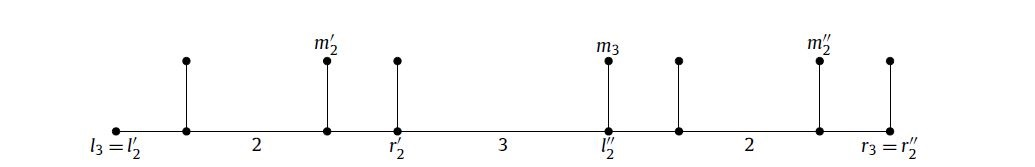
\includegraphics[width=12cm]{aa.JPG}
    \caption{Graph for construction Hurkens and Woeginger}
    \label{fig:graph2}
\end{figure}
% 
\begin{itemize}
% 
\item{Consider the graph by Hurkens and Woeginger}
\item{We will modify this structure according to our interest}
\item{
    We will:
    \begin{itemize}
        \item{Define a graph class $G_k$ for $k\geq1$}
        \item{Calculate parameters of the graph}
    \end{itemize}
}
% 
\end{itemize}
% 
} 
% 
% 
% 
\only<2->{
%
% 
% 
\begin{itemize}
% 
% 
    \only<2->{
        \item{Define three vertices on tree}
        \begin{itemize}
            \item {
                {\color{red}$l_k$} : Left most node of tree $G_k$ 
            }
            \item {
                {\color{red}$r_k$} : Right most node of tree $G_k$ 
            }
            \item {
                {\color{red}$m_k$} : Node connected to the right recursive portion's $l_k$ of  $G_k$ 
            }
        \end{itemize}
    }
% 
    \only<3->{
        \item{This will be a recursive graph}
        \item{Build graph for $G_1$}
        \begin{itemize}
            \item {
                Connect {\color{red}$l_1$} to {\color{red}$r_1$} with unit length edge 
            }
            \item {
                Connect {\color{red}$m_1$} to {\color{red}$r_1$} with unit length edge 
            }
        \end{itemize}
    }
% 
    \only<4->{
        \item{This will be a recursive graph}
        \item{Build graph for $G_k$}
        \item {
                Connect {\color{red}$G_{k-1}$} to {\color{red}$G'_{k-1}$} 
            }
        \begin{itemize}
            \item {
                Connect {\color{red}$r_{k-1}$} to {\color{red}$l'_{k-1}$} with edge of length $k$ 
            }
            \item {
                Connect {\color{red}$m_k$} to {\color{red}$r'_{k-1}$} with unit length edge 
            }
        \end{itemize}
        {\color{red}Construction of the graph is done!!}
    }
%     
\end{itemize} 
% 
}
% 
% 
% 
\end{frame}
% 
%
\subsection{Example of Constructed Tree}

\begin{frame}{Example of Constructed Tree}
    \begin{figure}
        
\begin{tikzpicture}[
        node/.style = {
            draw,
            circle,
            fill=gray,
            minimum size = #1,
            inner sep = 0pt,
            outer sep = 0pt
        },  
        node/.default = 6pt,
        node distance = {15mm}
    ]
    \only<1>{\node[node=10pt, label={[font=\large]below:$l_1$}, fill=orange] (1) {};}
    \only<1>{\node[node=10pt, label={[font=\large]below:$r_1$}, right of=1, fill=black!60!green] (2) {};}
    \only<1-2>{\node[node=10pt, label={[font=\large]right:$m_1$}, above of=2, fill=red] (3) {};}
    \draw[line width = 1pt] (1) -- node[above]{1} (2);
    \draw[line width = 1pt] (2) -- node[right]{1} (3);
    
    \only<1>{\node at (1, -1){\LARGE $G_1$};}
    \only<1>{\node at (5.6, -1){\LARGE $G_1$};}
    
    \only<1>{\node[node=10pt, label={[font=\large]below:$l_1'$}, fill=orange] (4) [right=30mm of 2] {};}
    \only<1>{\node[node=10pt, label={[font=\large]below:$r_1'$}, right of=4, fill=black!60!green] (5) {};}
    \only<1-2>{\node[node=10pt, label={[font=\large]right:$m_1'$}, above of=5, fill=red] (6) {};}
    \draw[line width = 1pt] (4) -- node[above]{1} (5);
    \draw[line width = 1pt] (5) -- node[right]{1} (6);\pause
    
    
    \node[node=10pt, label={[font=\large]below:$l_2$}, fill=orange] (1) {};
    \node[node=10pt, right of=1] (2) {};
    \node[node=10pt] (4) [right=30mm of 2] {};
    \node[node=10pt, label={[font=\large]below:$r_2$}, right of=4, fill=black!60!green] (5) {};
    \draw[line width = 1pt] (2) -- node[above]{2} (4);\pause
    
    \node[node=10pt, above of=2] (3) {};
    \node[node=10pt, above of=5] (6) {};
    \node[node=10pt, label={[font=\large]right:$m_2$}, fill=red, above of=4] (7) {};
    \draw[line width = 1pt, node distance = {20mm}] (4) -- node[right]{1} (7); 
    \node at (3.3, -1) {\LARGE $G_2$};
    
\end{tikzpicture}
        \label{fig:my_label}
    \end{figure}
    
\end{frame}

\begin{frame}{Example of Constructed Tree 2}
    \begin{figure}
        \centering
        \begin{tikzpicture}[
        node/.style = {
            fill=gray,
            draw,
            circle,
            fill,
            minimum size = #1,
            inner sep = 0pt,
            outer sep = 0pt
        },  
        node/.default = 6pt,
        node distance = {9mm}
    ]
    \only<1>{\node[node=10pt, label={[font=\large]below:$l_2$}, fill=orange] (1) {};}
    \node[node=10pt, right of=1] (2) {};
    \node[node=10pt, above of=2] (3) {};
    \node[node=10pt] (4) [right=18mm of 2] {};
    \only<1>{\node[node=10pt, label={[font=\large]below:$r_2$}, right of=4, fill=black!60!green] (5) {};}
    \node[node=10pt, above of=5] (6) {};
    \only<1-2>{\node[node=10pt, label={[font=\large]left:$m_2$}, above of=4, fill=red] (7) {};}
    
    \draw[line width = 1pt] (1) -- node[above]{1} (2);
    \draw[line width = 1pt] (2) -- node[right]{1} (3);
    \draw[line width = 1pt] (4) -- node[above]{1} (5);
    \draw[line width = 1pt] (5) -- node[right]{1} (6);
    \draw[line width = 1pt] (2) -- node[above]{2} (4);
    \draw[line width = 1pt] (4) -- node[right]{1} (7); 
    
    
    
    \only<1>{\node[node=10pt, label={[font=\large]below:$l_2'$}, fill=orange] (8) [right=27mm of 5] {};}
    \node[node=10pt, right of=8] (9) {};
    \node[node=10pt, above of=9] (10) {};
    \node[node=10pt] (11) [right=18mm of 9] {};
    \only<1>{\node[node=10pt, label={[font=\large]below:$r_2'$}, right of=11, fill=black!60!green] (12) {};}
    \node[node=10pt, above of=12] (13) {};
    \only<1-2>{\node[node=10pt, label={[font=\large]left:$m_2'$}, above of=11, fill=red] (14) {};}
    
    \draw[line width = 1pt] (8) -- node[above]{1} (9) ; 
    \draw[line width = 1pt] (9) -- node[right]{1} (10); 
    \draw[line width = 1pt] (9) -- node[above]{2} (11); 
    \draw[line width = 1pt] (11) -- node[above]{1} (12); 
    \draw[line width = 1pt] (12) -- node[right]{1} (13); 
    \draw[line width = 1pt] (11) -- node[right]{1} (14);\pause
    
    
    \node[node=10pt, label={[font=\large]below:$l_3$}, fill=orange] (1) {};
    \node[node=10pt, right of=4] (5) {};
    \node[node=10pt] (8) [right=27mm of 5] {};
    \node[node=10pt, label={[font=\large]below:$r_3$}, right of=11, fill=black!60!green] (12) {};
    \draw[line width = 1pt] (5) -- node[above]{3}  (8);\pause
    
    \node[node=10pt, above of=4] (7) {};
    \node[node=10pt, above of=11] (14) {};
    \node[node=10pt, label={[font=\large]left:$m_3$}, above of=8, fill=red] (15) {};
    \draw[line width = 1pt] (8) -- node[right]{1} (15);
    \node at (5.75, -1) {\LARGE $G_3$};
    
    
   
    
    
    
\end{tikzpicture}

        \label{fig:my_label}
    \end{figure}
\end{frame}
% 
\subsection{Parameters for Tree}
% 
% 
\begin{frame}{Parameters for Tree}
% 
    \only<1>{
    \begin{figure}[h]
        \centering
        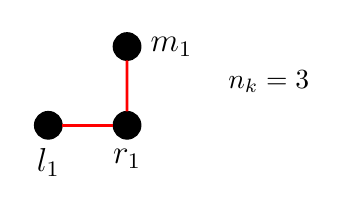
\begin{tikzpicture}[
            scale = 0.8,
            node/.style = {
                draw,
                circle,
                fill,
                minimum size = #1,
                inner sep = 0pt,
                outer sep = 0pt
            },  
            node/.default = 6pt,
            node distance = {10mm}
            ]
            \node[node=10pt, label={[font=\large]below:$l_1$}] (1) {};
            \node[node=10pt, label={[font=\large]below:$r_1$}, right of=1] (2) {};
            \node[node=10pt, label={[font=\large]right:$m_1$}, above of=2] (3) {};
            \draw[line width = 1pt, red] (1) -- (2);
            \draw[line width = 1pt, red] (2) -- (3);
            
            \node[] at (3.5,0.7) {$n_k=3$};
        \end{tikzpicture}
        \caption{Graph for $G_1$}
        \label{fig:graph1}
    \end{figure}
% 
%     
    We define {\color{ao(english}number of vertices} as {\color{red}$n_k$} 
    %
    \begin{itemize}
        \item {For $k = 1, {\color{red}n_k} = 3$ }
    \end{itemize} 
    }
    % 
    \only<2>{
    \begin{figure}[h]
        \centering
        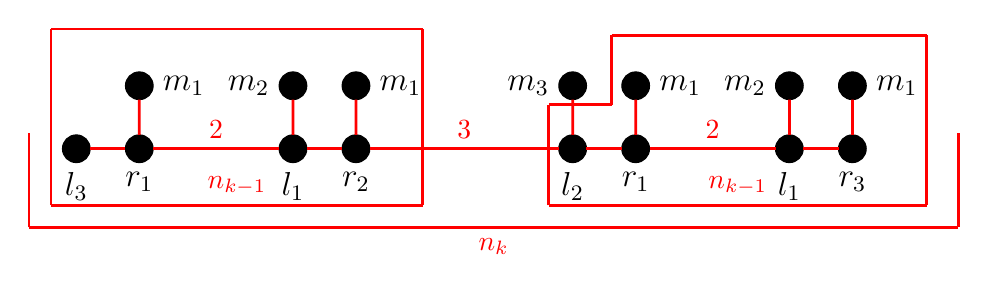
\begin{tikzpicture}[
                scale=0.8,
                node/.style = {
                    draw,
                    circle,
                    fill,
                    minimum size = #1,
                    inner sep = 0pt,
                    outer sep = 0pt
                },  
                node/.default = 6pt,
                node distance = {8mm}
            ]
            \node[node=10pt, label={[font=\large]below:$l_3$}] (1) {};
            \node[node=10pt, label={[font=\large]below:$r_1$}, right of=1] (2) {};
            \node[node=10pt, label={[font=\large]right:$m_1$}, above of=2] (3) {};
            % 
            \node[node=10pt, label={[font=\large]below:$l_1$}] (4) [right=16mm of 2] {};
            % 
            % 
            \node[node=10pt, label={[font=\large]below:$r_2$}, right of=4] (5) {};
            \node[node=10pt, label={[font=\large]right:$m_1$}, above of=5] (6) {};
            % 
            \node[node=10pt, label={[font=\large]left:$m_2$}, above of=4] (7) {};
            % 
            % 
            \node[node=10pt, label={[font=\large]below:$l_2$}] (8) [right=24mm of 5] {};
            \node[node=10pt, label={[font=\large]below:$r_1$}, right of=8] (9) {};
            \node[node=10pt, label={[font=\large]right:$m_1$}, above of=9] (10) {};
            % 
            \node[node=10pt, label={[font=\large]below:$l_1$}] (11) [right=16mm of 9] {};
            % 
            \node[node=10pt, label={[font=\large]below:$r_3$}, right of=11] (12) {};
            \node[node=10pt, label={[font=\large]right:$m_1$}, above of=12] (13) {};
            % 
            \node[node=10pt, label={[font=\large]left:$m_2$}, above of=11] (14) {};
            % 
            \node[node=10pt, label={[font=\large]left:$m_3$}, above of=8] (15) {};
            % 
            \draw[line width = 1pt, red] (1) -- (2);
            \draw[line width = 1pt, red] (2) -- (3);
            % 
            \draw[line width = 1pt, red] (4) -- (5);
            \draw[line width = 1pt, red] (5) -- (6);
            % 
            \draw[line width = 1pt, red] (2) -- node[above]{2} (4);
            \draw[line width = 1pt, red] (4) -- (7); 
            % 
            \draw[line width = 1pt, red] (8) -- (9) ; 
            \draw[line width = 1pt, red] (9) -- (10); 
            \draw[line width = 1pt, red] (9) -- node[above]{2} (11); 
            \draw[line width = 1pt, red] (11) -- (12); 
            \draw[line width = 1pt, red] (12) -- (13); 
            \draw[line width = 1pt, red] (11) -- (14);
            \draw[line width = 1pt, red] (5) -- node[above]{3}  (8);
            \draw[line width = 1pt, red] (8) -- (15);
            % 
            % 
            \draw[line width = 1pt, red] (-0.4,-0.9) -- node[above]{$n_{k-1}$} (5.5, -0.9);
            \draw[line width = 1pt, red] (-0.4, 1.9) -- (5.5, 1.9);
            \draw[line width = 1pt, red] (-0.4, -0.9) -- (-0.4, 1.9);
            \draw[line width = 1pt, red] (5.5, -0.9) -- (5.5, 1.9);
            % 
            \draw[line width = 1pt, red] (7.5,-0.9) -- node[above]{$n_{k-1}$} (13.5,-0.9);
            \draw[line width = 1pt, red] (8.5,1.8) -- (13.5, 1.8);
            \draw[line width = 1pt, red] (13.5, -0.9) -- (13.5,1.8);
            \draw[line width = 1pt, red] (8.5, 1.8) -- (8.5, 0.7);
            \draw[line width = 1pt, red] (7.5, -0.9) -- (7.5, 0.7);
            \draw[line width = 1pt, red] (7.5, 0.7) -- (8.5, 0.7);
            % 
            \draw[line width = 1pt, red] (-0.75,-1.25) -- node[below]{$n_{k}$} (14, -1.25);
            \draw[line width = 1pt, red] (14,-1.25) -- (14, 0.25);
            \draw[line width = 1pt, red] (-0.75, -1.25) -- (-0.75, 0.25);
            % 
        \end{tikzpicture}
        \caption{Graph for $G_3$}
        \label{fig:graph1}
    \end{figure}
% 
%     
    We define {\color{ao(english}number of vertices} as {\color{red}$n_k$} 
    %
    \begin{itemize}
        \item {For $k = 1, {\color{red}n_k} = 3$ }
        \item {For $k \geq 1, {\color{red}n_k} = 2*{\color{red}n_{k-1}} + 1$ }
    \end{itemize} 
% 
    It can be proved by induction that:
        $${\color{red}n_k} = 2^{k + 1} - 1$$
% 
    }
% 
%
\only<3>{
\begin{figure}[h]
        \centering
        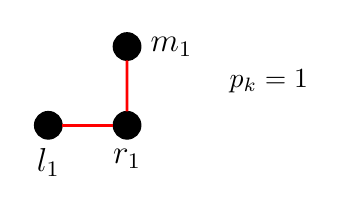
\begin{tikzpicture}[
            scale = 0.8,
            node/.style = {
                draw,
                circle,
                fill,
                minimum size = #1,
                inner sep = 0pt,
                outer sep = 0pt
            },  
            node/.default = 6pt,
            node distance = {10mm}
            ]
            \node[node=10pt, label={[font=\large]below:$l_1$}] (1) {};
            \node[node=10pt, label={[font=\large]below:$r_1$}, right of=1] (2) {};
            \node[node=10pt, label={[font=\large]right:$m_1$}, above of=2] (3) {};
            \draw[line width = 1pt, red] (1) -- (2);
            \draw[line width = 1pt, red] (2) -- (3);
            
            \node[] at (3.5,0.7) {$p_k=1$};
        \end{tikzpicture}
        \caption{Graph for $G_1$}
        \label{fig:graph1}
\end{figure}
% 
We define {\color{ao(english)}length} from {\color{red}$l_k$} to {\color{red}$r_k$} as {\color{red}$p_k$}  
\begin{itemize}
    \item {For $k=1, {\color{red}p_k}=1$  }
\end{itemize}
}

\only<4>{
    \begin{figure}[h]
        \centering
        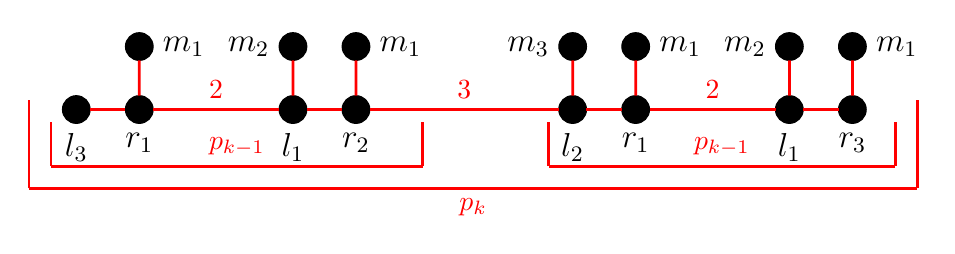
\begin{tikzpicture}[
                scale=0.8,
                node/.style = {
                    draw,
                    circle,
                    fill,
                    minimum size = #1,
                    inner sep = 0pt,
                    outer sep = 0pt
                },  
                node/.default = 6pt,
                node distance = {8mm}
            ]
            \node[node=10pt, label={[font=\large]below:$l_3$}] (1) {};
            \node[node=10pt, label={[font=\large]below:$r_1$}, right of=1] (2) {};
            \node[node=10pt, label={[font=\large]right:$m_1$}, above of=2] (3) {};
            % 
            \node[node=10pt, label={[font=\large]below:$l_1$}] (4) [right=16mm of 2] {};
            % 
            % 
            \node[node=10pt, label={[font=\large]below:$r_2$}, right of=4] (5) {};
            \node[node=10pt, label={[font=\large]right:$m_1$}, above of=5] (6) {};
            % 
            \node[node=10pt, label={[font=\large]left:$m_2$}, above of=4] (7) {};
            % 
            % 
            \node[node=10pt, label={[font=\large]below:$l_2$}] (8) [right=24mm of 5] {};
            \node[node=10pt, label={[font=\large]below:$r_1$}, right of=8] (9) {};
            \node[node=10pt, label={[font=\large]right:$m_1$}, above of=9] (10) {};
            % 
            \node[node=10pt, label={[font=\large]below:$l_1$}] (11) [right=16mm of 9] {};
            % 
            \node[node=10pt, label={[font=\large]below:$r_3$}, right of=11] (12) {};
            \node[node=10pt, label={[font=\large]right:$m_1$}, above of=12] (13) {};
            % 
            \node[node=10pt, label={[font=\large]left:$m_2$}, above of=11] (14) {};
            % 
            \node[node=10pt, label={[font=\large]left:$m_3$}, above of=8] (15) {};
            % 
            \draw[line width = 1pt, red] (1) -- (2);
            \draw[line width = 1pt, red] (2) -- (3);
            % 
            \draw[line width = 1pt, red] (4) -- (5);
            \draw[line width = 1pt, red] (5) -- (6);
            % 
            \draw[line width = 1pt, red] (2) -- node[above]{2} (4);
            \draw[line width = 1pt, red] (4) -- (7); 
            % 
            \draw[line width = 1pt, red] (8) -- (9) ; 
            \draw[line width = 1pt, red] (9) -- (10); 
            \draw[line width = 1pt, red] (9) -- node[above]{2} (11); 
            \draw[line width = 1pt, red] (11) -- (12); 
            \draw[line width = 1pt, red] (12) -- (13); 
            \draw[line width = 1pt, red] (11) -- (14);
            \draw[line width = 1pt, red] (5) -- node[above]{3}  (8);
            \draw[line width = 1pt, red] (8) -- (15);
            % 
            % 
            \draw[line width = 1pt, red] (-0.4,-0.9) -- node[above]{$p_{k-1}$} (5.5, -0.9);
            \draw[line width = 1pt, red] (-0.4, -0.9) -- (-0.4, -0.2);
            \draw[line width = 1pt, red] (5.5, -0.9) -- (5.5, -0.2);
            % 
            \draw[line width = 1pt, red] (7.5,-0.9) -- node[above]{$p_{k-1}$} (13,-0.9);
            \draw[line width = 1pt, red] (13, -0.9) -- (13,-0.2);
            \draw[line width = 1pt, red] (7.5, -0.9) -- (7.5, -0.2);
            % 
            \draw[line width = 1pt, red] (-0.75,-1.25) -- node[below]{$p_{k}$} (13.35, -1.25);
            \draw[line width = 1pt, red] (13.35,-1.25) -- (13.35, 0.15);
            \draw[line width = 1pt, red] (-0.75, -1.25) -- (-0.75, 0.15);
            % 
        \end{tikzpicture}
        \caption{Graph for $G_3$}
        \label{fig:graph1}
    \end{figure}
% 
We define {\color{ao(english)}length} from {\color{red}$l_k$} to {\color{red}$r_k$} as {\color{red}$p_k$}  
\begin{itemize}
    \item {For $k=1, {\color{red}p_k}=1$  }
    \item {For $k>1, {\color{red}p_k}=2*{\color{red}p_{k-1}}+k$  }
\end{itemize}
It can be proved by induction that: 
    $${\color{red}p_k}=2^{k+1}-k-2$$
% 
}
%
\only<5>{
 \begin{figure}[h]
        \centering
        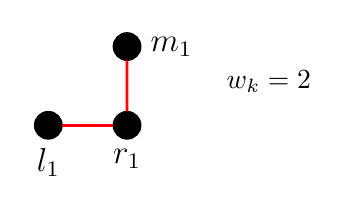
\begin{tikzpicture}[
            scale = 0.8,
            node/.style = {
                draw,
                circle,
                fill,
                minimum size = #1,
                inner sep = 0pt,
                outer sep = 0pt
            },  
            node/.default = 6pt,
            node distance = {10mm}
            ]
            \node[node=10pt, label={[font=\large]below:$l_1$}] (1) {};
            \node[node=10pt, label={[font=\large]below:$r_1$}, right of=1] (2) {};
            \node[node=10pt, label={[font=\large]right:$m_1$}, above of=2] (3) {};
            \draw[line width = 1pt, red] (1) -- (2);
            \draw[line width = 1pt, red] (2) -- (3);
            
            \node[] at (3.5,0.7) {$w_k=2$};
        \end{tikzpicture}
        \caption{Graph for $G_1$}
        \label{fig:graph1}
    \end{figure}
% 
We define {\color{ao(english)}sum of weights of all edges} from {\color{red}$l_k$} to {\color{red}$r_k$} as {\color{red}$w_k$}  
\begin{itemize}
    \item {For $k=1, {\color{red}w_k}=2$  }
\end{itemize}
}
\only<6>{
% 
    \begin{figure}[h]
        \centering
        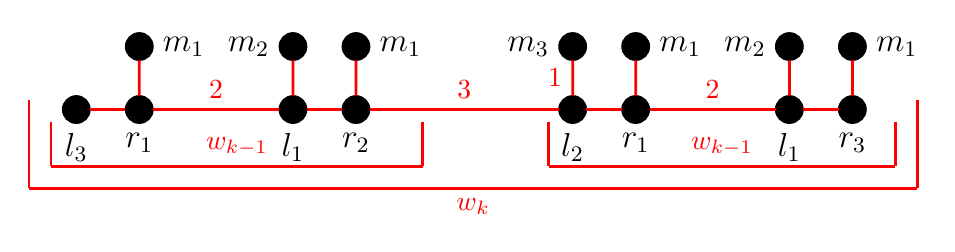
\begin{tikzpicture}[
                scale=0.8,
                node/.style = {
                    draw,
                    circle,
                    fill,
                    minimum size = #1,
                    inner sep = 0pt,
                    outer sep = 0pt
                },  
                node/.default = 6pt,
                node distance = {8mm}
            ]
            \node[node=10pt, label={[font=\large]below:$l_3$}] (1) {};
            \node[node=10pt, label={[font=\large]below:$r_1$}, right of=1] (2) {};
            \node[node=10pt, label={[font=\large]right:$m_1$}, above of=2] (3) {};
            % 
            \node[node=10pt, label={[font=\large]below:$l_1$}] (4) [right=16mm of 2] {};
            % 
            % 
            \node[node=10pt, label={[font=\large]below:$r_2$}, right of=4] (5) {};
            \node[node=10pt, label={[font=\large]right:$m_1$}, above of=5] (6) {};
            % 
            \node[node=10pt, label={[font=\large]left:$m_2$}, above of=4] (7) {};
            % 
            % 
            \node[node=10pt, label={[font=\large]below:$l_2$}] (8) [right=24mm of 5] {};
            \node[node=10pt, label={[font=\large]below:$r_1$}, right of=8] (9) {};
            \node[node=10pt, label={[font=\large]right:$m_1$}, above of=9] (10) {};
            % 
            \node[node=10pt, label={[font=\large]below:$l_1$}] (11) [right=16mm of 9] {};
            % 
            \node[node=10pt, label={[font=\large]below:$r_3$}, right of=11] (12) {};
            \node[node=10pt, label={[font=\large]right:$m_1$}, above of=12] (13) {};
            % 
            \node[node=10pt, label={[font=\large]left:$m_2$}, above of=11] (14) {};
            % 
            \node[node=10pt, label={[font=\large]left:$m_3$}, above of=8] (15) {};
            % 
            \draw[line width = 1pt, red] (1) -- (2);
            \draw[line width = 1pt, red] (2) -- (3);
            % 
            \draw[line width = 1pt, red] (4) -- (5);
            \draw[line width = 1pt, red] (5) -- (6);
            % 
            \draw[line width = 1pt, red] (2) -- node[above]{2} (4);
            \draw[line width = 1pt, red] (4) -- (7); 
            % 
            \draw[line width = 1pt, red] (8) -- (9) ; 
            \draw[line width = 1pt, red] (9) -- (10); 
            \draw[line width = 1pt, red] (9) -- node[above]{2} (11); 
            \draw[line width = 1pt, red] (11) -- (12); 
            \draw[line width = 1pt, red] (12) -- (13); 
            \draw[line width = 1pt, red] (11) -- (14);
            \draw[line width = 1pt, red] (5) -- node[above]{3}  (8);
            \draw[line width = 1pt, red] (8) -- node[left]{1} (15);
            % 
            % 
            \draw[line width = 1pt, red] (-0.4,-0.9) -- node[above]{$w_{k-1}$} (5.5, -0.9);
            \draw[line width = 1pt, red] (-0.4, -0.9) -- (-0.4, -0.2);
            \draw[line width = 1pt, red] (5.5, -0.9) -- (5.5, -0.2);
            % 
            \draw[line width = 1pt, red] (7.5,-0.9) -- node[above]{$w_{k-1}$} (13,-0.9);
            \draw[line width = 1pt, red] (13, -0.9) -- (13,-0.2);
            \draw[line width = 1pt, red] (7.5, -0.9) -- (7.5, -0.2);
            % 
            \draw[line width = 1pt, red] (-0.75,-1.25) -- node[below]{$w_{k}$} (13.35, -1.25);
            \draw[line width = 1pt, red] (13.35,-1.25) -- (13.35, 0.15);
            \draw[line width = 1pt, red] (-0.75, -1.25) -- (-0.75, 0.15);
            % 
        \end{tikzpicture}
        \caption{Graph for $G_3$}
        \label{fig:graph1}
    \end{figure}
%  
% 
We define {\color{ao(english)}sum of weights of all edges} from {\color{red}$l_k$} to {\color{red}$r_k$} as {\color{red}$w_k$}  
\begin{itemize}
    \item {For $k=1, {\color{red}w_k}=2$  }
    \item {For $k>1, {\color{red}w_k}=2*{\color{red}w_{k-1}}+k+1$  }
\end{itemize}
It can be proved by induction that: 
    $${\color{red}w_k}=3*2^{k}-k-3$$
% 
}
%
\only<7>{
% 
\begin{figure}[h]
        \centering
       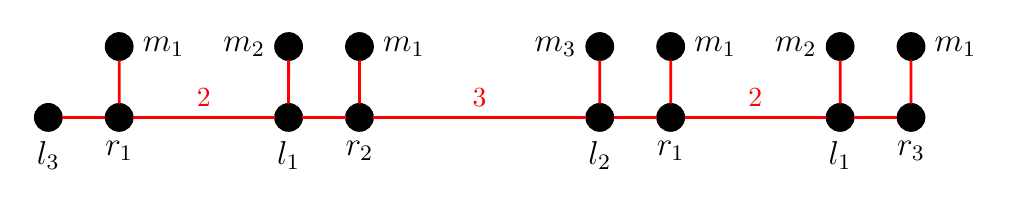
\begin{tikzpicture}[
        scale=0.8,
        node/.style = {
            draw,
            circle,
            fill,
            minimum size = #1,
            inner sep = 0pt,
            outer sep = 0pt
        },  
        node/.default = 6pt,
        node distance = {9mm}
    ]
    \node[node=10pt, label={[font=\large]below:$l_3$}] (1) {};
    \node[node=10pt, label={[font=\large]below:$r_1$}, right of=1] (2) {};
    \node[node=10pt, label={[font=\large]right:$m_1$}, above of=2] (3) {};
    
    \node[node=10pt, label={[font=\large]below:$l_1$}] (4) [right=18mm of 2] {};
    
    
    \node[node=10pt, label={[font=\large]below:$r_2$}, right of=4] (5) {};
    \node[node=10pt, label={[font=\large]right:$m_1$}, above of=5] (6) {};
    
    \node[node=10pt, label={[font=\large]left:$m_2$}, above of=4] (7) {};
    
    
    \node[node=10pt, label={[font=\large]below:$l_2$}] (8) [right=27mm of 5] {};
    \node[node=10pt, label={[font=\large]below:$r_1$}, right of=8] (9) {};
    \node[node=10pt, label={[font=\large]right:$m_1$}, above of=9] (10) {};
    
    \node[node=10pt, label={[font=\large]below:$l_1$}] (11) [right=18mm of 9] {};
    
    \node[node=10pt, label={[font=\large]below:$r_3$}, right of=11] (12) {};
    \node[node=10pt, label={[font=\large]right:$m_1$}, above of=12] (13) {};
    
    \node[node=10pt, label={[font=\large]left:$m_2$}, above of=11] (14) {};
    
    \node[node=10pt, label={[font=\large]left:$m_3$}, above of=8] (15) {};
    
    \draw[line width = 1pt, red] (1) -- (2);
    \draw[line width = 1pt, red] (2) -- (3);
    
    \draw[line width = 1pt, red] (4) -- (5);
    \draw[line width = 1pt, red] (5) -- (6);
    
    \draw[line width = 1pt, red] (2) -- node[above]{2} (4);
    \draw[line width = 1pt, red] (4) -- (7); 
    
    \draw[line width = 1pt, red] (8) -- (9) ; 
    \draw[line width = 1pt, red] (9) -- (10); 
    \draw[line width = 1pt, red] (9) -- node[above]{2} (11); 
    \draw[line width = 1pt, red] (11) --  (12); 
    \draw[line width = 1pt, red] (12) -- (13); 
    \draw[line width = 1pt, red] (11) -- (14);
    \draw[line width = 1pt, red] (5) -- node[above]{3}  (8);
    \draw[line width = 1pt, red] (8) -- (15);
    
\end{tikzpicture}
        \caption{Graph for $G_3$}
        \label{fig:graph1}
    \end{figure}
We define "{\color{ao(english)}optimal path weight} for the graph to start at {\color{red}$l_k$} and after visiting all the nodes, return to {\color{red}$l_k$}" as $OPT(G_k)$  
% 
\begin{align*}
    OPT(G_k)&=2*{\color{red}w_k} \\
            &=2*\left(3*2^{k}-k-3\right) \\
            &=6*2^{k}-2*k-6
\end{align*}
% 
}
% 
\only<8>{
% 
\begin{figure}[h]
        \centering
       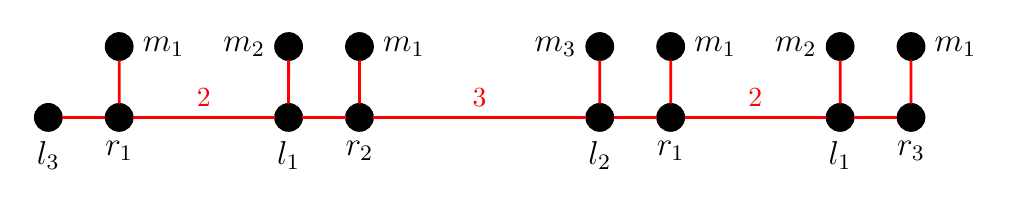
\begin{tikzpicture}[
        scale=0.8,
        node/.style = {
            draw,
            circle,
            fill,
            minimum size = #1,
            inner sep = 0pt,
            outer sep = 0pt
        },  
        node/.default = 6pt,
        node distance = {9mm}
            ]
            \node[node=10pt, label={[font=\large]below:$l_3$}] (1) {};
            \node[node=10pt, label={[font=\large]below:$r_1$}, right of=1] (2) {};
            \node[node=10pt, label={[font=\large]right:$m_1$}, above of=2] (3) {};
            
            \node[node=10pt, label={[font=\large]below:$l_1$}] (4) [right=18mm of 2] {};
            
            
            \node[node=10pt, label={[font=\large]below:$r_2$}, right of=4] (5) {};
            \node[node=10pt, label={[font=\large]right:$m_1$}, above of=5] (6) {};
            
            \node[node=10pt, label={[font=\large]left:$m_2$}, above of=4] (7) {};
            
            
            \node[node=10pt, label={[font=\large]below:$l_2$}] (8) [right=27mm of 5] {};
            \node[node=10pt, label={[font=\large]below:$r_1$}, right of=8] (9) {};
            \node[node=10pt, label={[font=\large]right:$m_1$}, above of=9] (10) {};
            
            \node[node=10pt, label={[font=\large]below:$l_1$}] (11) [right=18mm of 9] {};
            
            \node[node=10pt, label={[font=\large]below:$r_3$}, right of=11] (12) {};
            \node[node=10pt, label={[font=\large]right:$m_1$}, above of=12] (13) {};
            
            \node[node=10pt, label={[font=\large]left:$m_2$}, above of=11] (14) {};
            
            \node[node=10pt, label={[font=\large]left:$m_3$}, above of=8] (15) {};
            
            \draw[line width = 1pt, red] (1) -- (2);
            \draw[line width = 1pt, red] (2) -- (3);
            
            \draw[line width = 1pt, red] (4) -- (5);
            \draw[line width = 1pt, red] (5) -- (6);
            
            \draw[line width = 1pt, red] (2) -- node[above]{2} (4);
            \draw[line width = 1pt, red] (4) -- (7); 
            
            \draw[line width = 1pt, red] (8) -- (9) ; 
            \draw[line width = 1pt, red] (9) -- (10); 
            \draw[line width = 1pt, red] (9) -- node[above]{2} (11); 
            \draw[line width = 1pt, red] (11) -- (12); 
            \draw[line width = 1pt, red] (12) -- (13); 
            \draw[line width = 1pt, red] (11) -- (14);
            \draw[line width = 1pt, red] (5) -- node[above]{3}  (8);
            \draw[line width = 1pt, red] (8) -- (15);
            
        \end{tikzpicture}
        \caption{Graph for $G_3$}
        \label{fig:graph1}
    \end{figure}
{\color{ao(english)}Number of vertices}:\quad ${\color{red}n_k}=2^{k+1}-1$ 
\newline
%  
% 
{\color{ao(english)}Length} from {\color{red}$l_k$} to {\color{red}$r_k$}:
\quad ${\color{red}p_k}=2^{k+1}-k-2$
\newline
% 
% 
{\color{ao(english)}Sum of weights of all edges} from {\color{red}$l_k$} to {\color{red}$r_k$}:
\quad ${\color{red}w_k}=3*2^{k}-k-3$
\newline 
% 
% 
% 
\begin{columns}
%
\enskip
\begin{column}{0.55\textwidth}
{\color{ao(english)}Optimal path weight} for the graph to start at {\color{red}$l_k$} 
and after visiting all the nodes, return to {\color{red}$l_k$}:
\end{column} 
% 
% 
\begin{column}{0.45\textwidth}
    $OPT(G_k)=6*2^{k}-2*k-6$
\end{column}
% 
\end{columns}
% 
% 
}
% 
\end{frame}
% 
% 
% 
\subsection{Lemma 1}
% 
% 
% 
\begin{frame}{Lemma 1}
% 
\textbf{Lemma: }For {\color{red}$k\geq1$}, consider a graph {\color{red}$G$} that contains {\color{red}$G_k$} as a subgraph. Furthermore, assume that edges between {\color{red}$G_k$} and {\color{red}$G-G_k$} are either incident to {\color{red}$l_k$} and have a length of at least {\color{red}$1$} or are incident to {\color{red}$r_k$} and have a length of at least {\color{red}$k+1$}. \linebreak

{\qquad Then there exists a partial ${\color{red}NN}$ tour exploring all of {\color{red}$G_k$} that starts in {\color{red}$l_k$}, finishes in {\color{red}$m_k$} and has a length of {\color{red}$$(k+1)*2^k-2$$}}
\end{frame}
% 
% 
% 
% 
\begin{frame}{Proof of Lemma 1}
% 
% 
\only<1>{
% 
\begin{itemize}
    \item {
        edges between {\color{red}$G_k$} and {\color{red}$G-G_k$} are either incident to {\color{red}$l_k$} and have a length of at least {\color{red}$1$} or are incident to {\color{red}$r_k$} and have a length of at least {\color{red}$k+1$}
    }
\end{itemize}
% 
\begin{figure}[h]
    \centering
    % 
        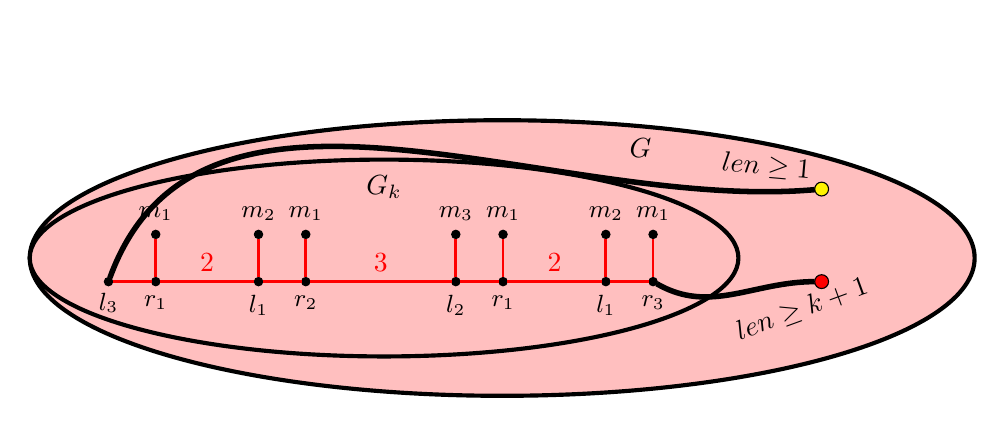
\begin{tikzpicture}[
                node/.style = {
                    draw,
                    circle,
                    fill,
                    minimum size = #1,
                    inner sep = 0pt,
                    outer sep = 0pt
                },  
                node/.default = 6pt,
                node distance = {6mm}
            ]
            
            % \draw[fill=pink] (3.5,0.4) ellipse (4.5cm and 1.5cm);
            \draw[fill=pink, line width=1.5pt] (10,0.4) arc [start angle=0, end angle=360, x radius=6cm, y radius=1.75cm]
                            node[pos=0.25, yshift=-1em, xshift=5em]{$G$};
            \draw[fill=pink, line width=1.5pt] (7,0.4) arc [start angle=0, end angle=360, x radius=4.5cm, y radius=1.25cm]
                            node[pos=0.25, yshift=-1em]{$G_k$};
            
            \node[node=3pt, label={[font=\small,yshift=0.1em]below:$l_3$}] (1) at (-1,0.1) {};
            \node[node=3pt, label={[font=\small]below:$r_1$}, right of=1] (2) {};
            \node[node=3pt, label={[font=\small]above:$m_1$}, above of=2] (3) {};
            
            \node[node=3pt, label={[font=\small]below:$l_1$}] (4) [right=12mm of 2] {};
            
            
            \node[node=3pt, label={[font=\small]below:$r_2$}, right of=4] (5) {};
            \node[node=3pt, label={[font=\small]above:$m_1$}, above of=5] (6) {};
            
            \node[node=3pt, label={[font=\small]above:$m_2$}, above of=4] (7) {};
            
            
            \node[node=3pt, label={[font=\small]below:$l_2$}] (8) [right=18mm of 5] {};
            \node[node=3pt, label={[font=\small]below:$r_1$}, right of=8] (9) {};
            \node[node=3pt, label={[font=\small]above:$m_1$}, above of=9] (10) {};
            
            \node[node=3pt, label={[font=\small]below:$l_1$}] (11) [right=12mm of 9] {};
            
            \node[node=3pt, label={[font=\small]below:$r_3$}, right of=11] (12) {};
            \node[node=3pt, label={[font=\small]above:$m_1$}, above of=12] (13) {};
            
            \node[node=3pt, label={[font=\small]above:$m_2$}, above of=11] (14) {};
            
            \node[node=3pt, label={[font=\small]above:$m_3$}, above of=8] (15) {};
            
        
            \node[node=5pt, fill=red] (G1) [right=20mm of 12]  {};
            \node[node=5pt, fill=yellow] (G2) [above=10mm of G1]  {};
            
            \draw[line width = 2pt] (1) to [out=70,in=185,looseness=0.95] (G2); 
            \draw[line width = 2pt] (12) to [out=-30,in=180,looseness=1] (G1); 
            
            \node[above of=G2, xshift=-2em, yshift = -0.9em, rotate = -5] {$len \geq 1$};
            \node[left of=G1, yshift = -1em, xshift = 1em, rotate = 20] {$len \geq k+1$};
            
            
            
            \draw[line width = 1pt, red] (1) -- (2);
            \draw[line width = 1pt, red] (2) -- (3);
            
            \draw[line width = 1pt, red] (4) -- (5);
            \draw[line width = 1pt, red] (5) -- (6);
            
            \draw[line width = 1pt, red] (2) -- node[above]{2} (4);
            \draw[line width = 1pt, red] (4) -- (7); 
            
            \draw[line width = 1pt, red] (8) -- (9) ; 
            \draw[line width = 1pt, red] (9) -- (10); 
            \draw[line width = 1pt, red] (9) -- node[above]{2} (11); 
            \draw[line width = 1pt, red] (11) --(12); 
            \draw[line width = 1pt, red] (12) --(13); 
            \draw[line width = 1pt, red] (11) --(14);
            \draw[line width = 1pt, red] (5) -- node[above]{3}  (8);
            \draw[line width = 1pt, red] (8) -- (15);
            
            
         \end{tikzpicture}
    % 
    \caption{Graph for Lemma 1}
    \label{fig:graph1}
\end{figure}
% 
}
% 
% 
\only<2>{
% 
\begin{figure}[h]
    \centering
    % 
    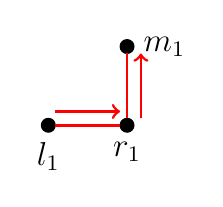
\begin{tikzpicture}[
        node/.style = {
                draw,
                circle,
                fill,
                minimum size = #1,
                inner sep = 0pt,
                outer sep = 0pt
            },  
            node/.default = 6pt,
            node distance = {10mm}
        ]
        \node[node=5pt, label={[font=\large]below:$l_1$}] (1) {};
        \node[node=5pt, label={[font=\large]below:$r_1$}, right of=1] (2) {};
        \node[node=5pt, label={[font=\large]right:$m_1$}, above of=2] (3) {};
        
        \draw[line width = 1pt, red] (1) -- (2);
        \draw[line width = 1pt, red] (2) -- (3);
        
        \draw[->, line width = 1pt, red, transform canvas={yshift=0.5em}] (1) -- (2);
        \draw[->, line width = 1pt, red, transform canvas={xshift=0.5em}] (2) -- (3);
        
    \end{tikzpicture}
    % 
    \caption{Condition for Lemma 1}
    \label{fig:graph1}
\end{figure}
% 
We prove this lemma by induction.
% 
\begin{itemize}
    \item {
        Let us consider graph {\color{red}$G_1$}
    } 
    \item {
        {\color{red}$l_1$} to {\color{red}$m_1$} path has length 3
    }
    \item {
        Satisfies the equation {\color{red}$(k+1)*2^k-2$} \\
        where ${\color{red}k = 1}$
    }
\end{itemize}
% 
} 
% 
\only<3-8>{
% 
% 
In {\color{red}$G_k$}, path starts at {\color{red}$l_k$}, finishes at {\color{red}$m_k$} and has a length of {\color{red}$(k+1)*2^k-2$} 
% 
% 
% 
\only<3>{
% 
    \begin{figure}[h]
        \centering
        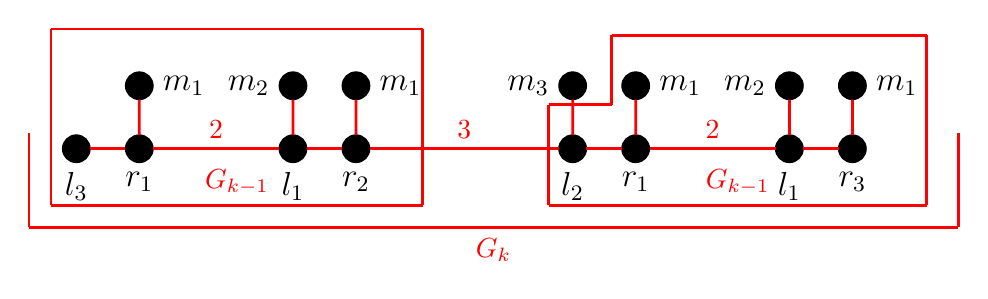
\begin{tikzpicture}[
                scale=0.8,
                node/.style = {
                    draw,
                    circle,
                    fill,
                    minimum size = #1,
                    inner sep = 0pt,
                    outer sep = 0pt
                },  
                node/.default = 6pt,
                node distance = {8mm}
            ]
            \node[node=10pt, label={[font=\large]below:$l_3$}] (1) {};
            \node[node=10pt, label={[font=\large]below:$r_1$}, right of=1] (2) {};
            \node[node=10pt, label={[font=\large]right:$m_1$}, above of=2] (3) {};
            % 
            \node[node=10pt, label={[font=\large]below:$l_1$}] (4) [right=16mm of 2] {};
            % 
            % 
            \node[node=10pt, label={[font=\large]below:$r_2$}, right of=4] (5) {};
            \node[node=10pt, label={[font=\large]right:$m_1$}, above of=5] (6) {};
            % 
            \node[node=10pt, label={[font=\large]left:$m_2$}, above of=4] (7) {};
            % 
            % 
            \node[node=10pt, label={[font=\large]below:$l_2$}] (8) [right=24mm of 5] {};
            \node[node=10pt, label={[font=\large]below:$r_1$}, right of=8] (9) {};
            \node[node=10pt, label={[font=\large]right:$m_1$}, above of=9] (10) {};
            % 
            \node[node=10pt, label={[font=\large]below:$l_1$}] (11) [right=16mm of 9] {};
            % 
            \node[node=10pt, label={[font=\large]below:$r_3$}, right of=11] (12) {};
            \node[node=10pt, label={[font=\large]right:$m_1$}, above of=12] (13) {};
            % 
            \node[node=10pt, label={[font=\large]left:$m_2$}, above of=11] (14) {};
            % 
            \node[node=10pt, label={[font=\large]left:$m_3$}, above of=8] (15) {};
            % 
            \draw[line width = 1pt, red] (1) -- (2);
            \draw[line width = 1pt, red] (2) -- (3);
            % 
            \draw[line width = 1pt, red] (4) -- (5);
            \draw[line width = 1pt, red] (5) -- (6);
            % 
            \draw[line width = 1pt, red] (2) -- node[above]{2} (4);
            \draw[line width = 1pt, red] (4) -- (7); 
            % 
            \draw[line width = 1pt, red] (8) -- (9) ; 
            \draw[line width = 1pt, red] (9) -- (10); 
            \draw[line width = 1pt, red] (9) -- node[above]{2} (11); 
            \draw[line width = 1pt, red] (11) -- (12); 
            \draw[line width = 1pt, red] (12) -- (13); 
            \draw[line width = 1pt, red] (11) -- (14);
            \draw[line width = 1pt, red] (5) -- node[above]{3}  (8);
            \draw[line width = 1pt, red] (8) -- (15);
            % 
            % 
            \draw[line width = 1pt, red] (-0.4,-0.9) -- node[above]{$G_{k-1}$} (5.5, -0.9);
            \draw[line width = 1pt, red] (-0.4, 1.9) -- (5.5, 1.9);
            \draw[line width = 1pt, red] (-0.4, -0.9) -- (-0.4, 1.9);
            \draw[line width = 1pt, red] (5.5, -0.9) -- (5.5, 1.9);
            % 
            \draw[line width = 1pt, red] (7.5,-0.9) -- node[above]{$G_{k-1}$} (13.5,-0.9);
            \draw[line width = 1pt, red] (8.5,1.8) -- (13.5, 1.8);
            \draw[line width = 1pt, red] (13.5, -0.9) -- (13.5,1.8);
            \draw[line width = 1pt, red] (8.5, 1.8) -- (8.5, 0.7);
            \draw[line width = 1pt, red] (7.5, -0.9) -- (7.5, 0.7);
            \draw[line width = 1pt, red] (7.5, 0.7) -- (8.5, 0.7);
            % 
            \draw[line width = 1pt, red] (-0.75,-1.25) -- node[below]{$G_{k}$} (14, -1.25);
            \draw[line width = 1pt, red] (14,-1.25) -- (14, 0.25);
            \draw[line width = 1pt, red] (-0.75, -1.25) -- (-0.75, 0.25);
            % 
        \end{tikzpicture}
        \caption{Graph for $G_3$}
        \label{fig:graph1}
    \end{figure}
\begin{itemize}
    \item {
        {\color{red}$G_k$} consists of two subgraph {\color{red}$G_{k-1}$} and {\color{red}$G_{k-1}'$}
    }
    \item {
        As this is proof by induction, we assume the conditions are met for the two subgraph {\color{red}$G_{k-1}$} and {\color{red}$G_{k-1}'$}
    }
% 
\end{itemize}
% 
}
% 
% 
\only<4>{
% 
% 
\begin{figure}[h]
    \centering
    % 
    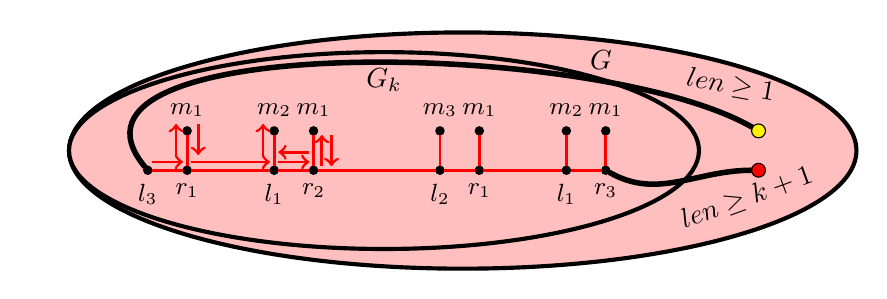
\begin{tikzpicture}[
        node/.style = {
            draw,
            circle,
            fill,
            minimum size = #1,
            inner sep = 0pt,
            outer sep = 0pt
        },  
        node/.default = 6pt,
        node distance = {5mm}
        ]
% 
        \draw[fill=pink, line width=1.5pt] (10,9) arc [start angle=0, end angle=360, x radius=5cm, y radius=1.5cm]
                        node[pos=0.25, yshift=-1em, xshift=5em]{$G$};
        \draw[fill=pink, line width=1.5pt] (8,9) arc [start angle=0, end angle=360, x radius=4cm, y radius=1.25cm]
                        node[pos=0.25, yshift=-1em]{$G_k$};
% 
         \node[node=3pt, label={[font=\small]below:$l_3$}] (1) at (1,8.75) {};
         \node[node=3pt, label={[font=\small]below:$r_1$}, right of=1] (2) {};
         \node[node=3pt, label={[font=\small]above:$m_1$}, above of=2] (3) {};
%  
        \node[node=3pt, label={[font=\small]below:$l_1$}] (4) [right=10mm of 2] {};
% 
% 
        \node[node=3pt, label={[font=\small]below:$r_2$}, right of=4] (5) {};
        \node[node=3pt, label={[font=\small]above:$m_1$}, above of=5] (6) {};
% 
        \node[node=3pt, label={[font=\small]above:$m_2$}, above of=4] (7) {};
% 
% 
        \node[node=3pt, label={[font=\small]below:$l_2$}] (8) [right=15mm of 5] {};
        \node[node=3pt, label={[font=\small]below:$r_1$}, right of=8] (9) {};
        \node[node=3pt, label={[font=\small]above:$m_1$}, above of=9] (10) {};
% 
        \node[node=3pt, label={[font=\small]below:$l_1$}] (11) [right=10mm of 9] {};
% 
        \node[node=3pt, label={[font=\small]below:$r_3$}, right of=11] (12) {};
        \node[node=3pt, label={[font=\small]above:$m_1$}, above of=12] (13) {};
% 
        \node[node=3pt, label={[font=\small]above:$m_2$}, above of=11] (14) {};
% 
        \node[node=3pt, label={[font=\small]above:$m_3$}, above of=8] (15) {};
% 
% 
        \node[node=5pt, fill=red] (G1) [right=18mm of 12]  {};
        \node[node=5pt, fill=yellow] (G2) [right=18mm of 13]  {};
% 
         \draw[line width = 2pt] (1) to [out=130,in=150,looseness=0.75] (G2); 
         \draw[line width = 2pt] (12) to [out=-30,in=180,looseness=1] (G1); 
% 
         \node[above of=G2, xshift=-1em, yshift = 0.2em, rotate = -10] {$len \geq 1$};
         \node[left of=G1, yshift = -1em, xshift = 1em, rotate = 20] {$len \geq k+1$};
% 
% 
% 
        \draw[line width = 1pt, red] (1) -- (2);
        \draw[line width = 1pt, red] (2) -- (3);
% 
        \draw[line width = 1pt, red] (4) -- (5);
        \draw[line width = 1pt, red] (5) -- (6);
% 
        \draw[line width = 1pt, red] (2) -- (4);
        \draw[line width = 1pt, red] (4) -- (7); 
% 
        \draw[line width = 1pt, red] (8) -- (9) ; 
        \draw[line width = 1pt, red] (9) -- (10); 
        \draw[line width = 1pt, red] (9) -- (11); 
        \draw[line width = 1pt, red] (11) --(12); 
        \draw[line width = 1pt, red] (12) --(13); 
        \draw[line width = 1pt, red] (11) --(14);
        \draw[line width = 1pt, red] (5) -- (8);
        \draw[line width = 1pt, red] (8) -- (15);
        
        \draw[->, line width = 1pt, red, transform canvas={yshift=0.3em}] (1) -- (2);
        \draw[->, line width = 1pt, red, transform canvas={xshift=-0.4em, yshift=0.4em}] (2) -- (3);
        \draw[->, line width = 1pt, red, transform canvas={xshift=0.4em, yshift=0.4em}] (3) -- (2);
        \draw[->, line width = 1pt, red, transform canvas={yshift=0.3em}] (2) -- (4);
        \draw[->, line width = 1pt, red, transform canvas={yshift=0.3em}] (4) -- (5);
        \draw[->, line width = 1pt, red, transform canvas={xshift=0.3em}] (5) -- (6);
        \draw[->, line width = 1pt, red, transform canvas={xshift=0.65em}] (6) -- (5);
        \draw[->, line width = 1pt, red, transform canvas={yshift=0.65em}] (5) -- (4);
        \draw[->, line width = 1pt, red, transform canvas={xshift=-0.4em, yshift=0.4em}] (4) -- (7);
        
    \end{tikzpicture}
    % 
    \caption{Traversal in $G_{k-1}$}
    \label{fig:my_label}
\end{figure}
\begin{itemize}
    \item {
        We start at {\color{red}$l_{k-1}$} in {\color{red}$G_{k-1}$} which is also {\color{red}$l_k$} for {\color{red}$G_k$} 
    }
    \item {
        We reach {\color{red}$m_{k-1}$} from {\color{red}$l_{k-1}$}
    }
    \item {
         path length: {\color{red}$k*2^{k-1}-2$} as {\color{red}$G_{k-1}$} satisfies the the lemma for {\color{red}$k-1$}
    }
    \item {
         {\color{red}$G_{k-1}$} graph traverse is done
    }
\end{itemize} 
% 
} 
% 
% 
% 
% 
\only<5>{
% 
We are at {\color{red}$m_{k-1}$}, we need to traverse subgraph {\color{red}$G_{k-1}'$} and then reach {\color{red}$m_{k}$}
% 
\begin{figure}
    \centering
    % 
    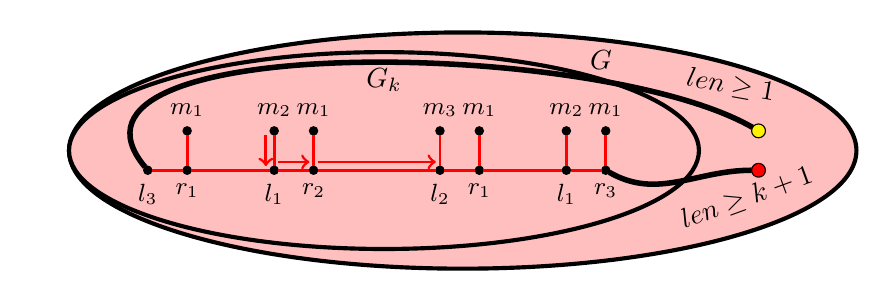
\begin{tikzpicture}[
        node/.style = {
            draw,
            circle,
            fill,
            minimum size = #1,
            inner sep = 0pt,
            outer sep = 0pt
        },  
        node/.default = 6pt,
        node distance = {5mm}
        ]
% 
        \draw[fill=pink, line width=1.5pt] (10,9) arc [start angle=0, end angle=360, x radius=5cm, y radius=1.5cm]
                        node[pos=0.25, yshift=-1em, xshift=5em]{$G$};
        \draw[fill=pink, line width=1.5pt] (8,9) arc [start angle=0, end angle=360, x radius=4cm, y radius=1.25cm]
                        node[pos=0.25, yshift=-1em]{$G_k$};
% 
         \node[node=3pt, label={[font=\small]below:$l_3$}] (1) at (1,8.75) {};
         \node[node=3pt, label={[font=\small]below:$r_1$}, right of=1] (2) {};
         \node[node=3pt, label={[font=\small]above:$m_1$}, above of=2] (3) {};
%  
        \node[node=3pt, label={[font=\small]below:$l_1$}] (4) [right=10mm of 2] {};
% 
% 
        \node[node=3pt, label={[font=\small]below:$r_2$}, right of=4] (5) {};
        \node[node=3pt, label={[font=\small]above:$m_1$}, above of=5] (6) {};
% 
        \node[node=3pt, label={[font=\small]above:$m_2$}, above of=4] (7) {};
% 
% 
        \node[node=3pt, label={[font=\small]below:$l_2$}] (8) [right=15mm of 5] {};
        \node[node=3pt, label={[font=\small]below:$r_1$}, right of=8] (9) {};
        \node[node=3pt, label={[font=\small]above:$m_1$}, above of=9] (10) {};
% 
        \node[node=3pt, label={[font=\small]below:$l_1$}] (11) [right=10mm of 9] {};
% 
        \node[node=3pt, label={[font=\small]below:$r_3$}, right of=11] (12) {};
        \node[node=3pt, label={[font=\small]above:$m_1$}, above of=12] (13) {};
% 
        \node[node=3pt, label={[font=\small]above:$m_2$}, above of=11] (14) {};
% 
        \node[node=3pt, label={[font=\small]above:$m_3$}, above of=8] (15) {};
% 
% 
        \node[node=5pt, fill=red] (G1) [right=18mm of 12]  {};
        \node[node=5pt, fill=yellow] (G2) [right=18mm of 13]  {};
% 
         \draw[line width = 2pt] (1) to [out=130,in=150,looseness=0.75] (G2); 
         \draw[line width = 2pt] (12) to [out=-30,in=180,looseness=1] (G1); 
% 
         \node[above of=G2, xshift=-1em, yshift = 0.2em, rotate = -10] {$len \geq 1$};
         \node[left of=G1, yshift = -1em, xshift = 1em, rotate = 20] {$len \geq k+1$};
% 
% 
% 
        \draw[line width = 1pt, red] (1) -- (2);
        \draw[line width = 1pt, red] (2) -- (3);
% 
        \draw[line width = 1pt, red] (4) -- (5);
        \draw[line width = 1pt, red] (5) -- (6);
% 
        \draw[line width = 1pt, red] (2) -- (4);
        \draw[line width = 1pt, red] (4) -- (7); 
% 
        \draw[line width = 1pt, red] (8) -- (9) ; 
        \draw[line width = 1pt, red] (9) -- (10); 
        \draw[line width = 1pt, red] (9) -- (11); 
        \draw[line width = 1pt, red] (11) --(12); 
        \draw[line width = 1pt, red] (12) --(13); 
        \draw[line width = 1pt, red] (11) --(14);
        \draw[line width = 1pt, red] (5) -- (8);
        \draw[line width = 1pt, red] (8) -- (15);
        
        \draw[->, line width = 1pt, red, transform canvas={xshift=-0.3em}] (7) -- (4);
        \draw[->, line width = 1pt, red, transform canvas={yshift=0.3em}] (4) -- (5);
        \draw[->, line width = 1pt, red, transform canvas={yshift=0.3em}] (5) -- (8);
        
    \end{tikzpicture}
    % 
    \caption{$m_{k-1}$ to $l_{k-1}'$}
    \label{fig:my_label}
\end{figure}
% 
\begin{itemize}
    \item {
        We can go outside of {\color{red}$G_{k-1}$} and then traverse {\color{red}$G_{k-1}'$} independently
        % 
        \begin{itemize}
            \item {
                Through {\color{red}$l_{k-1}$}, length at least
                {\color{red}$1 + k + p_{k-2}$}
            }
            \item {
                Through {\color{red}$r_{k-1}$}, length at least 
                {\color{red}$1 + p_{k-2} + k$}
            }
        \end{itemize}
    }
    \item {
        We can go straight to {\color{red}$l_{k-1}'$}, length: 
        {\color{red}$1 + p_{k-2} + k $}
    }
\end{itemize} 
% 
We choose going to {\color{red}$l_{k-1}'$}
} 
% 
%
\only<6>{
% 
\begin{figure}
    \centering
    %
    
    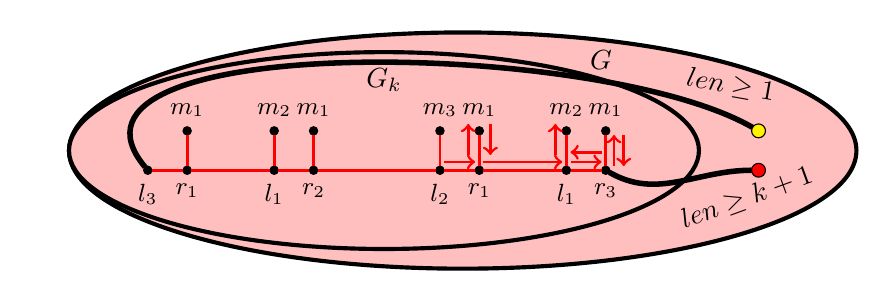
\begin{tikzpicture}[
        node/.style = {
            draw,
            circle,
            fill,
            minimum size = #1,
            inner sep = 0pt,
            outer sep = 0pt
        },  
        node/.default = 6pt,
        node distance = {5mm}
        ]
% 
        \draw[fill=pink, line width=1.5pt] (10,9) arc [start angle=0, end angle=360, x radius=5cm, y radius=1.5cm]
                        node[pos=0.25, yshift=-1em, xshift=5em]{$G$};
        \draw[fill=pink, line width=1.5pt] (8,9) arc [start angle=0, end angle=360, x radius=4cm, y radius=1.25cm]
                        node[pos=0.25, yshift=-1em]{$G_k$};
% 
         \node[node=3pt, label={[font=\small]below:$l_3$}] (1) at (1,8.75) {};
         \node[node=3pt, label={[font=\small]below:$r_1$}, right of=1] (2) {};
         \node[node=3pt, label={[font=\small]above:$m_1$}, above of=2] (3) {};
%  
        \node[node=3pt, label={[font=\small]below:$l_1$}] (4) [right=10mm of 2] {};
% 
% 
        \node[node=3pt, label={[font=\small]below:$r_2$}, right of=4] (5) {};
        \node[node=3pt, label={[font=\small]above:$m_1$}, above of=5] (6) {};
% 
        \node[node=3pt, label={[font=\small]above:$m_2$}, above of=4] (7) {};
% 
% 
        \node[node=3pt, label={[font=\small]below:$l_2$}] (8) [right=15mm of 5] {};
        \node[node=3pt, label={[font=\small]below:$r_1$}, right of=8] (9) {};
        \node[node=3pt, label={[font=\small]above:$m_1$}, above of=9] (10) {};
% 
        \node[node=3pt, label={[font=\small]below:$l_1$}] (11) [right=10mm of 9] {};
% 
        \node[node=3pt, label={[font=\small]below:$r_3$}, right of=11] (12) {};
        \node[node=3pt, label={[font=\small]above:$m_1$}, above of=12] (13) {};
% 
        \node[node=3pt, label={[font=\small]above:$m_2$}, above of=11] (14) {};
% 
        \node[node=3pt, label={[font=\small]above:$m_3$}, above of=8] (15) {};
% 
% 
        \node[node=5pt, fill=red] (G1) [right=18mm of 12]  {};
        \node[node=5pt, fill=yellow] (G2) [right=18mm of 13]  {};
% 
         \draw[line width = 2pt] (1) to [out=130,in=150,looseness=0.75] (G2); 
         \draw[line width = 2pt] (12) to [out=-30,in=180,looseness=1] (G1); 
% 
         \node[above of=G2, xshift=-1em, yshift = 0.2em, rotate = -10] {$len \geq 1$};
         \node[left of=G1, yshift = -1em, xshift = 1em, rotate = 20] {$len \geq k+1$};
% 
% 
% 
        \draw[line width = 1pt, red] (1) -- (2);
        \draw[line width = 1pt, red] (2) -- (3);
% 
        \draw[line width = 1pt, red] (4) -- (5);
        \draw[line width = 1pt, red] (5) -- (6);
% 
        \draw[line width = 1pt, red] (2) -- (4);
        \draw[line width = 1pt, red] (4) -- (7); 
% 
        \draw[line width = 1pt, red] (8) -- (9) ; 
        \draw[line width = 1pt, red] (9) -- (10); 
        \draw[line width = 1pt, red] (9) -- (11); 
        \draw[line width = 1pt, red] (11) --(12); 
        \draw[line width = 1pt, red] (12) --(13); 
        \draw[line width = 1pt, red] (11) --(14);
        \draw[line width = 1pt, red] (5) -- (8);
        \draw[line width = 1pt, red] (8) -- (15);
        
        \draw[->, line width = 1pt, red, transform canvas={yshift=0.3em}] (8) -- (9);
        \draw[->, line width = 1pt, red, transform canvas={xshift=-0.4em, yshift=0.4em}] (9) -- (10);
        \draw[->, line width = 1pt, red, transform canvas={xshift=0.4em, yshift=0.4em}] (10) -- (9);
        \draw[->, line width = 1pt, red, transform canvas={yshift=0.3em}] (9) -- (11);
        \draw[->, line width = 1pt, red, transform canvas={yshift=0.3em}] (11) -- (12);
        \draw[->, line width = 1pt, red, transform canvas={xshift=0.3em}] (12) -- (13);
        \draw[->, line width = 1pt, red, transform canvas={xshift=0.65em}] (13) -- (12);
        \draw[->, line width = 1pt, red, transform canvas={yshift=0.65em}] (12) -- (11);
        \draw[->, line width = 1pt, red, transform canvas={xshift=-0.4em, yshift=0.4em}] (11) -- (14);
        
    \end{tikzpicture}
    %
    \caption{Caption}
    \label{fig:my_label}
\end{figure}
% 
\begin{itemize}
    \item {
        We are at {\color{red}$l_{k-1}'$} in {\color{red}$G_{k-1}'$}
    }
    \item {
        We reach {\color{red}$m_{k-1}'$} from {\color{red}$l_{k-1}'$}
    }
    \item {
         path length: {\color{red}$k*2^{k-1}-2$} as {\color{red}$G_{k-1}'$} satisfies the the lemma for {\color{red}$k-1$}
    }
    \item {
         {\color{red}$G_{k-1}'$} graph traverse is done
    }
\end{itemize} 
% 
} 
%  
% 
\only<7>{
% 
% 
\begin{figure}
    \centering
    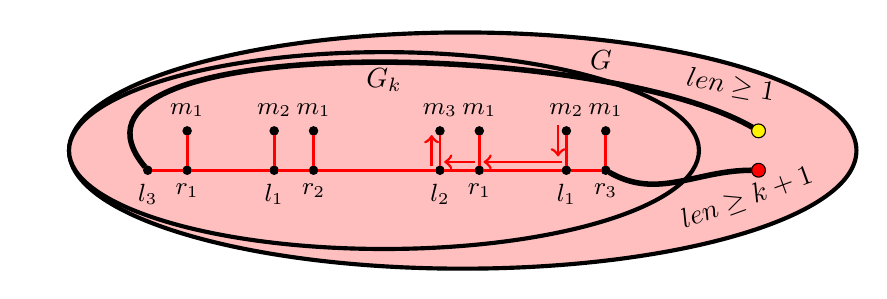
\begin{tikzpicture}[
        node/.style = {
            draw,
            circle,
            fill,
            minimum size = #1,
            inner sep = 0pt,
            outer sep = 0pt
        },  
        node/.default = 6pt,
        node distance = {5mm}
        ]
% 
        \draw[fill=pink, line width=1.5pt] (10,9) arc [start angle=0, end angle=360, x radius=5cm, y radius=1.5cm]
                        node[pos=0.25, yshift=-1em, xshift=5em]{$G$};
        \draw[fill=pink, line width=1.5pt] (8,9) arc [start angle=0, end angle=360, x radius=4cm, y radius=1.25cm]
                        node[pos=0.25, yshift=-1em]{$G_k$};
% 
         \node[node=3pt, label={[font=\small]below:$l_3$}] (1) at (1,8.75) {};
         \node[node=3pt, label={[font=\small]below:$r_1$}, right of=1] (2) {};
         \node[node=3pt, label={[font=\small]above:$m_1$}, above of=2] (3) {};
%  
        \node[node=3pt, label={[font=\small]below:$l_1$}] (4) [right=10mm of 2] {};
% 
% 
        \node[node=3pt, label={[font=\small]below:$r_2$}, right of=4] (5) {};
        \node[node=3pt, label={[font=\small]above:$m_1$}, above of=5] (6) {};
% 
        \node[node=3pt, label={[font=\small]above:$m_2$}, above of=4] (7) {};
% 
% 
        \node[node=3pt, label={[font=\small]below:$l_2$}] (8) [right=15mm of 5] {};
        \node[node=3pt, label={[font=\small]below:$r_1$}, right of=8] (9) {};
        \node[node=3pt, label={[font=\small]above:$m_1$}, above of=9] (10) {};
% 
        \node[node=3pt, label={[font=\small]below:$l_1$}] (11) [right=10mm of 9] {};
% 
        \node[node=3pt, label={[font=\small]below:$r_3$}, right of=11] (12) {};
        \node[node=3pt, label={[font=\small]above:$m_1$}, above of=12] (13) {};
% 
        \node[node=3pt, label={[font=\small]above:$m_2$}, above of=11] (14) {};
% 
        \node[node=3pt, label={[font=\small]above:$m_3$}, above of=8] (15) {};
% 
% 
        \node[node=5pt, fill=red] (G1) [right=18mm of 12]  {};
        \node[node=5pt, fill=yellow] (G2) [right=18mm of 13]  {};
% 
         \draw[line width = 2pt] (1) to [out=130,in=150,looseness=0.75] (G2); 
         \draw[line width = 2pt] (12) to [out=-30,in=180,looseness=1] (G1); 
% 
         \node[above of=G2, xshift=-1em, yshift = 0.2em, rotate = -10] {$len \geq 1$};
         \node[left of=G1, yshift = -1em, xshift = 1em, rotate = 20] {$len \geq k+1$};
% 
% 
% 
        \draw[line width = 1pt, red] (1) -- (2);
        \draw[line width = 1pt, red] (2) -- (3);
% 
        \draw[line width = 1pt, red] (4) -- (5);
        \draw[line width = 1pt, red] (5) -- (6);
% 
        \draw[line width = 1pt, red] (2) -- (4);
        \draw[line width = 1pt, red] (4) -- (7); 
% 
        \draw[line width = 1pt, red] (8) -- (9) ; 
        \draw[line width = 1pt, red] (9) -- (10); 
        \draw[line width = 1pt, red] (9) -- (11); 
        \draw[line width = 1pt, red] (11) --(12); 
        \draw[line width = 1pt, red] (12) --(13); 
        \draw[line width = 1pt, red] (11) --(14);
        \draw[line width = 1pt, red] (5) -- (8);
        \draw[line width = 1pt, red] (8) -- (15);
        
        \draw[->, line width = 1pt, red, transform canvas={xshift=-0.3em, yshift=0.35em}] (14) -- (11);
        \draw[->, line width = 1pt, red, transform canvas={yshift=0.3em}] (11) -- (9);
        \draw[->, line width = 1pt, red, transform canvas={yshift=0.3em}] (9) -- (8);
        \draw[->, line width = 1pt, red, transform canvas={xshift=-0.3em}] (8) -- (15);
        
    \end{tikzpicture}
    \caption{$m_{k-1}'$ to $m_k$}
    \label{fig:my_label}
\end{figure}
% 
Now, only {\color{red}$m_k$} vertex traversal is left, we are at {\color{red}$m_{k-1}'$}
% 
\begin{itemize}
    \item {
        We can go outside of {\color{red}$G_{k}$} and then reach {\color{red}$m_k$} independently
        % 
        \begin{itemize}
            \item {
                Through {\color{red}$l_{k-1}$}, length at least
                {\color{red}$1 + 3*k + 3*p_{k-2}$}
            }
            \item {
                Through {\color{red}$r_{k-1}'$}, length at least 
                {\color{red}$2 + p_{k-2} + k$}
            }
        \end{itemize}
    }
    \item {
        We can go straight to {\color{red}$m_k$} through {\color{red}$l_{k-1}'$}, length: 
        {\color{red}$1 + k + p_{k-2} $}
    }
\end{itemize} 
% 
Obviously, we choose to reach straight to {\color{red}$m_k$}
% 
} 
% 
% 
\only<8>{
% 
\begin{figure}
    \centering
    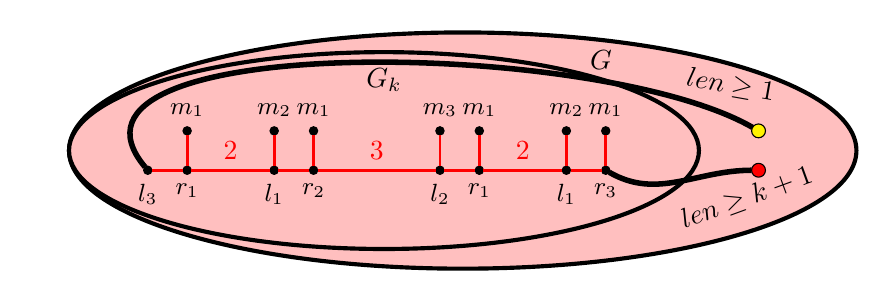
\begin{tikzpicture}[
        node/.style = {
            draw,
            circle,
            fill,
            minimum size = #1,
            inner sep = 0pt,
            outer sep = 0pt
        },  
        node/.default = 6pt,
        node distance = {5mm}
        ]
% 
        \draw[fill=pink, line width=1.5pt] (10,9) arc [start angle=0, end angle=360, x radius=5cm, y radius=1.5cm]
                        node[pos=0.25, yshift=-1em, xshift=5em]{$G$};
        \draw[fill=pink, line width=1.5pt] (8,9) arc [start angle=0, end angle=360, x radius=4cm, y radius=1.25cm]
                        node[pos=0.25, yshift=-1em]{$G_k$};
% 
         \node[node=3pt, label={[font=\small]below:$l_3$}] (1) at (1,8.75) {};
         \node[node=3pt, label={[font=\small]below:$r_1$}, right of=1] (2) {};
         \node[node=3pt, label={[font=\small]above:$m_1$}, above of=2] (3) {};
%  
        \node[node=3pt, label={[font=\small]below:$l_1$}] (4) [right=10mm of 2] {};
% 
% 
        \node[node=3pt, label={[font=\small]below:$r_2$}, right of=4] (5) {};
        \node[node=3pt, label={[font=\small]above:$m_1$}, above of=5] (6) {};
% 
        \node[node=3pt, label={[font=\small]above:$m_2$}, above of=4] (7) {};
% 
% 
        \node[node=3pt, label={[font=\small]below:$l_2$}] (8) [right=15mm of 5] {};
        \node[node=3pt, label={[font=\small]below:$r_1$}, right of=8] (9) {};
        \node[node=3pt, label={[font=\small]above:$m_1$}, above of=9] (10) {};
% 
        \node[node=3pt, label={[font=\small]below:$l_1$}] (11) [right=10mm of 9] {};
% 
        \node[node=3pt, label={[font=\small]below:$r_3$}, right of=11] (12) {};
        \node[node=3pt, label={[font=\small]above:$m_1$}, above of=12] (13) {};
% 
        \node[node=3pt, label={[font=\small]above:$m_2$}, above of=11] (14) {};
% 
        \node[node=3pt, label={[font=\small]above:$m_3$}, above of=8] (15) {};
% 
% 
        \node[node=5pt, fill=red] (G1) [right=18mm of 12]  {};
        \node[node=5pt, fill=yellow] (G2) [right=18mm of 13]  {};
% 
         \draw[line width = 2pt] (1) to [out=130,in=150,looseness=0.75] (G2); 
         \draw[line width = 2pt] (12) to [out=-30,in=180,looseness=1] (G1); 
% 
         \node[above of=G2, xshift=-1em, yshift = 0.2em, rotate = -10] {$len \geq 1$};
         \node[left of=G1, yshift = -1em, xshift = 1em, rotate = 20] {$len \geq k+1$};
% 
% 
% 
        \draw[line width = 1pt, red] (1) -- (2);
        \draw[line width = 1pt, red] (2) -- (3);
% 
        \draw[line width = 1pt, red] (4) -- (5);
        \draw[line width = 1pt, red] (5) -- (6);
% 
        \draw[line width = 1pt, red] (2) -- node[above]{2} (4);
        \draw[line width = 1pt, red] (4) -- (7); 
% 
        \draw[line width = 1pt, red] (8) -- (9) ; 
        \draw[line width = 1pt, red] (9) -- (10); 
        \draw[line width = 1pt, red] (9) -- node[above]{2} (11); 
        \draw[line width = 1pt, red] (11) --(12); 
        \draw[line width = 1pt, red] (12) --(13); 
        \draw[line width = 1pt, red] (11) --(14);
        \draw[line width = 1pt, red] (5) -- node[above]{3}  (8);
        \draw[line width = 1pt, red] (8) -- (15);
    \end{tikzpicture}
    \caption{Graph for $G_k$}
    \label{fig:my_label}
\end{figure}
% 
We have completed our traversal from {\color{red}$l_k$} to {\color{red}$m_k$}.
Total length of the path:
\begin{itemize}
    \item {
        {\color{red}$l_k$} to {\color{red}$m_{k-1}$} in subgraph {\color{red}$G_{k-1}$}:
            {\color{ao(english)}$k*2^{k-1}-2$}
    }
    \item {
        {\color{red}$m_{k-1}$} to {\color{red}$l_{k-1}'$}:
            {\color{ao(english)}$1+k+p_{k-2}$}
    }
    \item {
        {\color{red}$l_{k-1}'$} to {\color{red}$m_{k-1}'$} in subgraph {\color{red}$G_{k-1}'$}:
            {\color{ao(english)}$k*2^{k-1}-2$}
    }
    \item {
        {\color{red}$m_{k-1}'$} to {\color{red}$m_k$}:
            {\color{ao(english)}$1+k+p_{k-2}$}
    }
\end{itemize}
% 
}
% 
}
% 
\only<9>{
% 
Total length of whole traversal:
% 
\begin{align*}
    L_k &= 2*(1+k+p_{k-2}) + 2*(k*2^{k-1}-2) \\
        &= 2 + 2k + 2p_{k-2} + 2k*2^{k-1} - 4 \\
        &= 2k - 2 + 2k*2^{k-1} + 2p_{k-2} \\
        &= 2k - 2 + 2k*2^{k-1} + 2(2^{k-1} - (k-2) - 2) \\
        &= 2k - 2 + k*2^k + 2^k - 2k + 4 - 4 \\
        &= 2^k(k + 1) - 2 \qed
\end{align*}
% 
}
% 
\end{frame}
% 
% 
% 
%  
% 
% 
% 
%  
\subsection{Competitive Ratio for Trees}
% 
% 
\begin{frame}{Competitive Ratio of Trees}
% 
\only<1>{
Our goal was to show that the "{\color{ao(english)}tighter bounds of competitive ratio of NN}" also holds on the family of the tree.    
\begin{itemize}
    \item {
        The upper bound follows directly from the general case.   
    }
    \item {
        We show that: The lower bound on trees remains same if we follow {\color{red}$NN$} approach.
    }
\end{itemize} 
}
%
% 
\only<2->{
% 
Calculating the Competitive Ratio lower bound: 
%
% 
\only<2>{
% 
%
\begin{itemize}
        \item {
            Traversing graph {\color{red}$G_k$} when {\color{red}$G_k$} is a part of larger graph {\color{red}$G$} with some conditions, the shortest path length from {\color{red}$l_k$} to {\color{red}$m_k$} is {\color{red}$(k+1)*2^k-2$}. \qquad [Lemma 1]
        }
        \item {
            We can use Lemma 1 for only {\color{red}$G_k$} as we did not need to go outside {\color{red}$G_k$} in Lemma 1.
        }
        \item {
            Finally complete exploration by returning to {\color{red}$l_k$} from {\color{red}$m_k$}.
        }
    \end{itemize}
% 
} 
% 
%
\only<3>{
% 
\begin{figure}
    \centering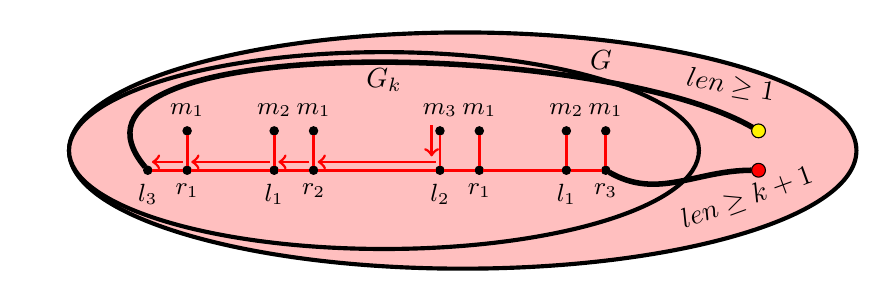
\begin{tikzpicture}[
        node/.style = {
            draw,
            circle,
            fill,
            minimum size = #1,
            inner sep = 0pt,
            outer sep = 0pt
        },  
        node/.default = 6pt,
        node distance = {5mm}
        ]
% 
        \draw[fill=pink, line width=1.5pt] (10,9) arc [start angle=0, end angle=360, x radius=5cm, y radius=1.5cm]
                        node[pos=0.25, yshift=-1em, xshift=5em]{$G$};
        \draw[fill=pink, line width=1.5pt] (8,9) arc [start angle=0, end angle=360, x radius=4cm, y radius=1.25cm]
                        node[pos=0.25, yshift=-1em]{$G_k$};
% 
         \node[node=3pt, label={[font=\small]below:$l_3$}] (1) at (1,8.75) {};
         \node[node=3pt, label={[font=\small]below:$r_1$}, right of=1] (2) {};
         \node[node=3pt, label={[font=\small]above:$m_1$}, above of=2] (3) {};
%  
        \node[node=3pt, label={[font=\small]below:$l_1$}] (4) [right=10mm of 2] {};
% 
% 
        \node[node=3pt, label={[font=\small]below:$r_2$}, right of=4] (5) {};
        \node[node=3pt, label={[font=\small]above:$m_1$}, above of=5] (6) {};
% 
        \node[node=3pt, label={[font=\small]above:$m_2$}, above of=4] (7) {};
% 
% 
        \node[node=3pt, label={[font=\small]below:$l_2$}] (8) [right=15mm of 5] {};
        \node[node=3pt, label={[font=\small]below:$r_1$}, right of=8] (9) {};
        \node[node=3pt, label={[font=\small]above:$m_1$}, above of=9] (10) {};
% 
        \node[node=3pt, label={[font=\small]below:$l_1$}] (11) [right=10mm of 9] {};
% 
        \node[node=3pt, label={[font=\small]below:$r_3$}, right of=11] (12) {};
        \node[node=3pt, label={[font=\small]above:$m_1$}, above of=12] (13) {};
% 
        \node[node=3pt, label={[font=\small]above:$m_2$}, above of=11] (14) {};
% 
        \node[node=3pt, label={[font=\small]above:$m_3$}, above of=8] (15) {};
% 
% 
        \node[node=5pt, fill=red] (G1) [right=18mm of 12]  {};
        \node[node=5pt, fill=yellow] (G2) [right=18mm of 13]  {};
% 
         \draw[line width = 2pt] (1) to [out=130,in=150,looseness=0.75] (G2); 
         \draw[line width = 2pt] (12) to [out=-30,in=180,looseness=1] (G1); 
% 
         \node[above of=G2, xshift=-1em, yshift = 0.2em, rotate = -10] {$len \geq 1$};
         \node[left of=G1, yshift = -1em, xshift = 1em, rotate = 20] {$len \geq k+1$};
% 
% 
% 
        \draw[line width = 1pt, red] (1) -- (2);
        \draw[line width = 1pt, red] (2) -- (3);
% 
        \draw[line width = 1pt, red] (4) -- (5);
        \draw[line width = 1pt, red] (5) -- (6);
% 
        \draw[line width = 1pt, red] (2) -- (4);
        \draw[line width = 1pt, red] (4) -- (7); 
% 
        \draw[line width = 1pt, red] (8) -- (9) ; 
        \draw[line width = 1pt, red] (9) -- (10); 
        \draw[line width = 1pt, red] (9) -- (11); 
        \draw[line width = 1pt, red] (11) --(12); 
        \draw[line width = 1pt, red] (12) --(13); 
        \draw[line width = 1pt, red] (11) --(14);
        \draw[line width = 1pt, red] (5) -- (8);
        \draw[line width = 1pt, red] (8) -- (15);
        
        \draw[->, line width = 1pt, red, transform canvas={xshift=-0.3em, yshift=0.35em}] (15) -- (8);
        \draw[->, line width = 1pt, red, transform canvas={yshift=0.3em}] (8) -- (5);
        \draw[->, line width = 1pt, red, transform canvas={yshift=0.3em}] (5) -- (4);
        \draw[->, line width = 1pt, red, transform canvas={yshift=0.3em}] (4) -- (2);
        \draw[->, line width = 1pt, red, transform canvas={yshift=0.3em}] (2) -- (1);
        
    \end{tikzpicture}

    \caption{$m_k$ to $l_k$}
    \label{fig:my_label}
\end{figure}
% 
    \begin{itemize}
        \item {
            {\color{red}$l_k$} to {\color{red}$m_k$} needs length: \qquad {\color{red}$(k+1)*2^k-2$}      
        }
        \item {
            {\color{red}$m_k$} to {\color{red}$l_k$} needs length: 
            \begin{align*}
                Ret(G_k)    &= 1 + k + p_{k-1} \\
                            &= 1 + k + (2^k - (k-1) - 2) \\
                            &= 1 + k + 2^k - k + 1 - 2 = 2^k 
            \end{align*}
        }
    \end{itemize}
% 
} 
% 
% 
\only<4>{
    \begin{itemize}
        \item {
            Total length for complete exploration on Online Tree {\color{red}$G_k$}: 
            \begin{align*}
                NN(G_k) &= Ret(G_k) + (k+1)*2^k - 2 \\
                        &= 2^k + (k+1)*2^k - 2 \\
                        &= (k+2)*2^k - 2 \\
            \end{align*}
        }
    \end{itemize}
} 
% 
% 
\only<5>{
\begin{itemize}
    \item {
        The {\color{ao(english)}NN} approach on particular Online Tree family has length: 
            $$(k+2)*2^k-2$$
    }
    \item {
        The optimal solution on this offline Tree family should have length: 
            \begin{align*}
                OPT(G_k) &= 2*w_k \\
                         &= 6*2^k - 2k - 6
            \end{align*}
    }
    \item {
          {\color{red}$G_k$} has vertices:
          \begin{align*}
              n_k &= 2^{k+1}-1 \\ 
              2^{k+1} &= n_k + 1 \\ 
              log_2{2^{k+1}} &= log_2{(n_k + 1)} \\ 
              k + 1 &= log_2{(n_k + 1)} \\ 
              k &= log_2{(n_k + 1)} - 1 
          \end{align*}
    }
\end{itemize}
}
% 
% 
\only<6>{
    \begin{itemize}
    \item {
        Lower bound: 
        \begin{align*}
            c   &= \frac{NN(G_k)}{OPT(G_k)} \\
                &= \frac{(k+2)*2^k - 2}{6*2^k - 2k - 6} \\
                &\geq \frac{k+2}{6} \\
                &= \frac{\log_2{(n+1)}+1}{6} \qed  
        \end{align*}
    }
    \end{itemize}
} 
} 
% 
% 
% 
% 
% 
%    
\end{frame} 
\begin{frame}
\begin{center}
{\fontsize{40}{50}\selectfont Thank You!}
\end{center}
\end{frame}

% 
% 
% 
% 
% 
% 
\end{document}